
% Define as main tex file
% !TEX root = Optimization.tex

%%%%%%%%%%%%%%%%%%%%%%%%%%%%%%%%%%%%%%%%%
% Dokumentinformationen
%%%%%%%%%%%%%%%%%%%%%%%%%%%%%%%%%%%%%%%%%
\newcommand{\titleinfo}{Optimization}
\newcommand{\authorinfo}{R. Koller, G. Danuser, S.Eicher} % Do not remove any names! Initial authors stay first.
\newcommand{\versioninfo}{FS2013}

%%%%%%%%%%%%%%%%%%%%%%%%%%%%%%%%%%%%%%%%%
% Standard projektübergreifender Header
%%%%%%%%%%%%%%%%%%%%%%%%%%%%%%%%%%%%%%%%%
% Genereller Header
\documentclass[10pt,twoside,a4paper,fleqn]{article}
\usepackage[utf8]{inputenc}
\usepackage[left=1cm,right=1cm,top=1cm,bottom=1cm,includeheadfoot]{geometry}
\usepackage[ngerman]{babel,varioref}
\usepackage[T1]{fontenc}

% Pakete
\usepackage{amssymb}
\usepackage{amsmath}
\usepackage{bm} %bold math symbols
\usepackage{fancybox}
\usepackage{graphicx}
\usepackage{color}
\usepackage{xcolor}
\usepackage{lastpage}
\usepackage{wrapfig}
\usepackage{fancyhdr}
\usepackage{hyperref}
\usepackage{tikz}
\usepackage{verbatim}
\usepackage{floatflt}
\usepackage{arydshln}
\usepackage{ucs}
\usepackage{pdflscape} % landscape
\usepackage{multirow} % zellen in tabellen verbinden
\usepackage{multicol}
%s\usepackage{diagbox} % getrennte zelle in tabelle
% \usepackage{array} % anordnung in tabellen

%%%%%%%%%%%%%%%%%%%%
% Generelle Makros %
%%%%%%%%%%%%%%%%%%%%
\newcommand{\formelbuch}[1]{$_{\textcolor{red}{\mbox{\small{S#1}}}}$}
\newcommand{\verweis}[2]{ {\small (siehe auch \ref{#1}, #2 (S. \pageref{#1}))
}}
\newcommand{\subsubadd}[1]{\textcolor{black}{\mbox{#1}}}
\newenvironment{liste}[0]{
	\begin{list}{$\bullet$}{\setlength{\itemsep}{0cm}\setlength{\parsep}{0cm} \setlength{\topsep}{0cm}}}
    {\end{list}}

\newcommand{\logd}[0]{\log_{10}}
\newcommand{\subsubsubsection}[1]{\textbf{#1}}

\newenvironment{aufzaehlung}[0]{
	\begin{enumerate}{\setlength{\itemsep}{0cm}\setlength{\parsep}{0cm}
	\setlength{\topsep}{0cm}}} {\end{enumerate}}

\newcommand{\abbHeight}[3]{
	\begin{center}
		\includegraphics[height=#2]{./bilder/#1} \\
		#3
    \end{center}
}

%\newcommand{\skriptsection}[2]{\section{#1 {\tiny Skript S. #2}}}
%\newcommand{\skriptsubsection}[2]{\subsection{#1 {\tiny Skript S. #2}}}
%\newcommand{\skriptsubsubsection}[2]{\subsubsection{#1 {\tiny Skript S. #2}}}
%\renewcommand{\skriptsection}[2]{\section{#1 {\tiny Schaum S. #2}}}
%\renewcommand{\skriptsubsection}[2]{\subsection{#1 {\tiny Schaum S. #2}}}
%\renewcommand{\skriptsubsubsection}[2]{\subsubsection{#1 {\tiny Schaum S. #2}}}
\newcommand{\skriptsection}[2]{\section{#1 \formelbuch{#2}}}
\newcommand{\skriptsubsection}[2]{\subsection{#1 \formelbuch{#2}}}
\newcommand{\skriptsubsubsection}[2]{\subsubsection{#1 \formelbuch{#2}}}

%%%%%%%%%%
% Farben %
%%%%%%%%%%
\definecolor{black}{rgb}{0,0,0}
\definecolor{red}{rgb}{1,0,0}
\definecolor{white}{rgb}{1,1,1}
\definecolor{grey}{rgb}{0.8,0.8,0.8}

%%%%%%%%%%%%%%%%%%%%%%%%%%%%
% Mathematische Operatoren %
%%%%%%%%%%%%%%%%%%%%%%%%%%%%
\DeclareMathOperator{\sinc}{sinc}
\DeclareMathOperator{\sgn}{sgn}
\DeclareMathOperator{\tr}{tr}
\DeclareMathOperator{\tridiag}{tridiag}



% Fouriertransformationen
\unitlength1cm
\newcommand{\FT}
{
\begin{picture}(1,0.5)
\put(0.2,0.1){\circle{0.14}}\put(0.27,0.1){\line(1,0){0.5}}\put(0.77,0.1){\circle*{0.14}}
\end{picture}
}


\newcommand{\IFT}
{
\begin{picture}(1,0.5)
\put(0.2,0.1){\circle*{0.14}}\put(0.27,0.1){\line(1,0){0.45}}\put(0.77,0.1){\circle{0.14}}
\end{picture}
}

\newcommand{\todo}[1]{\colorbox{red}{\textbf{#1}}}
\newcommand{\e}{\mathrm{e}}
\newcommand{\grad}[1]{\underset{#1}{\mathrm{grad~}}}
\DeclareMathOperator{\Real}{Re}
\DeclareMathOperator{\Imag}{Im}

\newcommand{\cfbox}[2]{%
    \colorlet{currentcolor}{.}%
    {\color{#1}%
    \fbox{\color{currentcolor}#2}}%
}


\newcommand{\partFrac}[2]{\frac{\partial #1}{\partial #2}}

%%%%%%%%%%%%%%%%%%%%%%%%%%%%
% Allgemeine Einstellungen %
%%%%%%%%%%%%%%%%%%%%%%%%%%%%
%pdf info
\hypersetup{pdfauthor={\authorinfo},pdftitle={\titleinfo},colorlinks=false}
\author{\authorinfo}
\title{\titleinfo}

%Kopf- und Fusszeile
\pagestyle{fancy}
\fancyhf{}
%Linien oben und unten
\renewcommand{\headrulewidth}{0.5pt}
\renewcommand{\footrulewidth}{0.5pt}


\fancyhead[L]{\titleinfo{ }- Summary}
%Kopfzeile rechts bzw. aussen
\fancyhead[R]{\today{ }- Page \thepage/\pageref{LastPage}}
\fancyfoot[C]{\copyright{ }\authorinfo}

% Einr�cken verhindern versuchen
\setlength{\parindent}{0pt}


\begin{document}
%%%%%%%%%%%%%%%%%%%%%%%%%%%%%%%%%%%%%%%%%
% Dokument
%%%%%%%%%%%%%%%%%%%%%%%%%%%%%%%%%%%%%%%%%

\maketitle
\tableofcontents
\clearpage

\section{Mathematische Modelle \skript{27}}
\subsection{Deskriptive Modelle und Optimierungsmodelle \skript{27}}
  \begin{tabular}{|p{3.7cm}|p{7cm}|p{7cm}|}
    \hline
    & \textbf{Deskriptive Modelle}
    & \textbf{Optimierungsmodelle} \\
    \hline
    \hline
    Antworten auf\ldots
      & ``What if?''
      & ``What's best?'' \\
    \hline
    Mengen ($I$)
      & \multicolumn{2}{l|}{Typen von Objekten (z.B. Städte $I = \{1,2,\ldots,n\}$)} \\
    \hline
    Parameter ($p_i$)
      & \multicolumn{2}{p{14cm}|}{Vorgegebene Grössen des Modells (z.B. aktueller Fahrzeugbestand in Filiale $i$, Distanz zwischen Filiale $i$ und $j$)} \\
    \hline
    Variablen ($x_{ij}$)
      & \multicolumn{2}{l|}{Veränderbare Modellgrösse (z.B. Anz. transferierte Fahrzeuge von Filiale $i$ nach $j$)} \\
    \hline
    Konsequenzen ($k_{i}, k_i^{out}$)
      & Output des deskriptiven Modells (z.B. gesamte Fahrdistanz), $k_0 = f_0(x,p)$ 
      & -\\
    \hline
    Zielfunktion $\min$ oder $\max$
      & - 
      & Zu maximierende oder minimierende Konsequenz\\
    \hline
    Restriktionen / Constraints ($k_{i}, k_i^{out}$)
      & - 
      & Bedingungen auf den Konsequenzen (Ungleichungen, selten Gleichungen) ACHTUNG: 'Idiotische' Bedingungen nicht vergessen: Keine negativen Mengen produzieren, etc.\\
    \hline
  \end{tabular}
  
  \subsubsection{Beispiel für Modellierung: Warenverteilung (Ähnlich, aber nicht identisch zu Klinkerts Mietwagenvermietung, Übung 1, Aufgabe 2 bzw. \skript{23})}
  Eine Ware soll von Lagern an Filialen ausgeliefert werden mit minimalen Transportkosten.\\
  
  \textbf{Mengen:}\\
  \begin{tabular}{lll}
    $I$ & Menge der Lager, &$I = \{1, \ldots, m\}$\\
    $J$ & Menge der Filialen, &$J = \{1, \ldots, n\}$
  \end{tabular}\\
  
  \textbf{Parameter:}\\
  \begin{tabular}{lll}
    $a_{i}$ & Lagerbestand der Ware in Lager $i$& $i \in I$ \\
    $b_j$   & Bedarf der Filiale $j$& $j \in J$\\
    $c_{ij}$& Kosten für Beförderung von Lager $i$ nach Filiale $j$& $i \in I, j \in J$\\
  \end{tabular}\\
  
  \textbf{Variablen:}\\
  \begin{tabular}{lll}
    $x_{ij}$ & Verschobene Menge von $i$ nach $j$ & $i \in I, j \in J$\\
  \end{tabular}\\
  
  \textbf{Zielfunktion:}\\
  \begin{tabular}{l}
    min $\sum\limits_{i \in I,~j \in J}c_{ij} x_{ij}$\\
  \end{tabular}\\
  
  \textbf{Restriktionen:}\\
  \begin{tabular}{lll}
    $\sum\limits_{j \in J}x_{ij}\leq a_{i}$ & $i \in I$          & (Nicht mehr Waren ausliefern als im Lager vorhanden)\\
    $\sum\limits_{i \in I}x_{ij}\geq b_{j}$ & $j \in J$          & (Nicht weniger Waren ausliefern als benötigt)\\
    $x_{ij} \ge 0$                          & $i \in I, j \in J$ & (Nicht negative Anzahl Waren ausliefern)\\
  \end{tabular}\\
  
  \subsubsection{Beispiel für Modellierung: Legierungen (Klinkert, Übung 4, Aufgabe 5)}
    Aus den Edelmetallen $I$ sollen die Legierungen $J$ gemischt werden. Der Erlös soll maximiert werden.\\
    
    \textbf{Mengen:}\\
    \begin{tabular}{lll}
      $I$ & Menge der Edelmetalle, &$I = \{1, \ldots, m\}$\\
      $J$ & Menge der Legierungen, &$J = \{1, \ldots, n\}$
    \end{tabular}\\

    \textbf{Parameter:}\\
    \begin{tabular}{lll}
      $a_{ij}$ & Menge von Edelmetall $i$ pro Menge Legierung $j$ & $i \in I, j \in J$\\
      $b_i$    & Verfügbare Menge von Edelmetall $i$              & $i \in I$\\
      $c_j$    & Erlös pro Menge Legierung $j$                    & $j \in J$\\
    \end{tabular}\\

    \textbf{Variablen:}\\
    \begin{tabular}{lll}
      $x_j$ & Produktionsmenge von Legierung $j$ & $j \in J$\\
    \end{tabular}\\

    \textbf{Zielfunktion:}\\
    \begin{tabular}{l}
      max $\sum\limits_{j \in J}c_j x_j$\\
    \end{tabular}\\

    \textbf{Restriktionen:}\\
    \begin{tabular}{lll}
      $\sum\limits_{j \in J}a_{ij}x_j \le b_i$ & $i \in I$ & (nicht mehr Legierung produzieren als Edelmetall vorhanden)\\
      $x_j \ge 0$                       & $j \in J$ & (nicht negative Mengen Legierungen produzieren)
    \end{tabular}\\




\subsection{Allgemeines Optimierungsproblem \skript{31}}
  In Form von Ungleichungen und Gleichungen werden mögliche Lösungsmengen (\em solution spaces\em) definiert. Dort soll eine Zielfunktion $f$ optimiert (maximiert oder minimiert) werden. Die Fragestellung lautet: "`What's best?"' (preskriptive Modelle).
  
  \begin{center}
    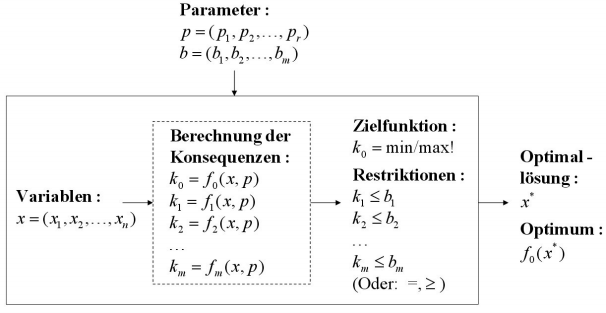
\includegraphics[width=10cm]{./Content/OptMathModels/OptimiziationModel}
  \end{center}
  
  \begin{tabularx}{\textwidth}{p{7cm} X}
  \hline
    \textbf{Problemformulierung} & \\
  \hline
    Allgemeines Optimierungsproblem
      & $\Pi: \max\{f(x) : x \in S\}$ wobei $S \subseteq \mathbb{R}^n$\\
    Entscheidungsvariablen/Variablen (\em decision variables/variables\em)
      & Vektor $x = (x_1, ..., x_n) \in \mathbb{R}^n$\\
    Lösungsmenge/Lösungsraum (\em solution space, feasible region\em)
      & $S$ von $\Pi$\\
    Zielfunktion
      & $f: S \rightarrow \mathbb{R}$\\
    Zulässigkeit (\em feasibility\em)
      & Lösungsraum darf nicht leer sein ($S \neq 0$)\\
    Beschränktheit (\em boundedness\em)
      & $f(x) \leq \omega,\, \omega \in \mathbb{R}$ für alle $x \in S$\\
    Abgeschlossenheit (\em closedness\em)
      & Zusätzlich zu Zulässigkeit und Beschränktheit: $x^* \in S$ (Optimallösung existiert)\\
    Kontinuität (\em continuity\em)
      & \(f\) ist eine kontinuierliche Funktion \\
  \hline
    \textbf{Definition des Lösungsraums} & \\
  \hline
    Funktionale Restriktionen (\em functional constraints\em)
      & $p\geq 0$ Ungleichungen der Form $g_i(x) \leq 0$, \newline
        $q \geq 0$ Ungleichungen der Form $h_j(x) = 0$.\newline
        $g_i(x), h_j(x)$ sind lineare Funktionen!\\
    Nicht-funktionale Restriktionen 
      & Definition des Lösungsraums $S$ durch "`nicht-funktionale"' Restriktionen, z.B. logische Prädikate (z.B. $S=\{x \in \mathbb{Z}^n: x \text{ ist eine Permutation der Zahlen } 1,...,n \}$) \\
  \hline
    \textbf{Maximierungs-/Minimierungsprobleme} & Beides möglich, Umwandlung siehe \ref{sec:linprog_umwandlungen}\\
  \hline
    Extremwert-Theorem von Weierstrasse
      & Wenn $S \subseteq \mathbb{R}^n$ eine nichtleere, begrenzte, abgeschlossene Menge und $f: S \rightarrow \mathbb{R}$ eine stetige Funktion ist, existiert ein $x^* \in S$ mit $f(x^*) \geq f(x)$
       für alle $x \in S$, d.h. das Optimierungsproblem hat eine Optimallösung.\\
  \hline
    \textbf{Nachbarschaft (\em Neighbourhood\em)} & Beliebige Menge Punkte "`in der Nähe"' des aktuellen Punktes $x$\\
  \hline
    Euklidische Nachbarschaft
      & $N_\epsilon(x) = \{ y \in \mathbb{R}^n: ||y-x|| \leq \varepsilon \}$ mit $\varepsilon > 0$, $||x|| = \sqrt{x^2} = \sqrt{x_1^2 + ... + x_n^2}$ (in $\mathbb{R}^2$ ein Kreis, $\mathbb{R}^3$ eine Kugel, etc.)\\
    Andere Nachbarschaften
      & Es sind auch andere Nachbarschaftsdefinitionen möglich (ohne Bsp.)\\
  \hline
    \textbf{Diverses} &\\
  \hline
      Globale Optimallösung
      & $x^*$ ist eine globale Optimallösung wenn $f(x^*) \geq f(x)$ für alle $x \in S$.\\
    Lokale Optima
      & $x^*$ ist eine lokale Optimallösung (bzgl. Nachbarschaft $N_\varepsilon$) wenn $f(x^*) \geq f(x)$ für alle $x \in N_\varepsilon(x^*) \cap S$\\
    Niveaumengen (Höhenlinien, \em level sets\em)
      & Orthogonale Linien zu den linearen Funktionen (Geraden)\\      
  \end{tabularx}
  

\subsection{Konvexe Optimierung \skript{40}}
  \begin{tabularx}{\textwidth}{p{6cm} X}
  \hline
    \textbf{Definitionen} & \\
  \hline
    $\lambda$
      & $\lambda \in \mathbb{R}$ mit $0 \leq \lambda \leq 1$\\
    Konvexkombination zweier Vektoren
      & $x^1, x^2 \in \mathbb{R}^n$:  $x = \lambda x^1 + (1-\lambda) x^2$ \\
    Konvexe Funktion
      & $f(\lambda x^1 + (1-\lambda)x^2) \leq \lambda f(x^1) + (1-\lambda)f(x^2)$ für alle $x^1, x^2 \in S$, $S$ konvex \newline
      Deutsch: Lineare Interpolation zwischen $x^1$ und $x^2$ ist kleiner gleich als Funktion\\
    Konkave Funktion
      & $f(\lambda x^1 + (1-\lambda)x^2) \geq \lambda f(x^1) + (1-\lambda)f(x^2)$ für alle $x^1, x^2 \in S$, $S$ konvex \newline
      Deutsch: Lineare Interpolation zwischen $x^1$ und $x^2$ ist grösser gleich als Funktion\\
    Lineare Funktion
      & Eine lineare Funktion ist sowohl konvex als auch konkav in $S$.\\
    Konvexe Menge
      & $\lambda x^1 + (1-\lambda)x^2 \in S$ für Vektoren $x^1,x^2 \in S \subseteq \mathbb{R}^n, \lambda \in \mathbb{R}, 0 \leq \lambda \leq 1$.\newline
      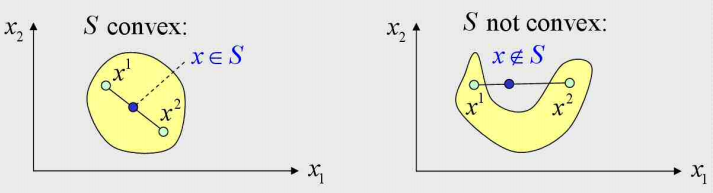
\includegraphics[width=7cm]{./Content/OptMathModels/ConvexSet} \\
    Konvexes Optimierungsproblem
      & Ein konvexes Optimierungsproblem ist \em entweder \em die Maximierung einer konkaven Funktion $f$ über einer konvexen Menge $S$ \em oder \em die Minimierung einer konvexen Funktion $f$ über einer konvexen Menge $S$.\\
  \hline  
    \textbf{Eigenschaften} & \\
  \hline
    Globales Optimum
      & In einem konvexen Optimierungsproblem ist jedes lokale Optimum ein globales Optimum! \\
    Optimum auf Rand
      & $S \subseteq \mathbb{R}^n$ sei eine konvexe, abgeschlossene, begrenzte Menge. Bei einem Optimierungsproblem der Form $\max\{ f(x) : x \in S \}$ (bzw. $\min\{ f(x) : x \in S \}$) mit $f$ konvex (bzw. konkav) in $S$ liegt jede lokale Optimallösung auf dem Rand. \newline 
      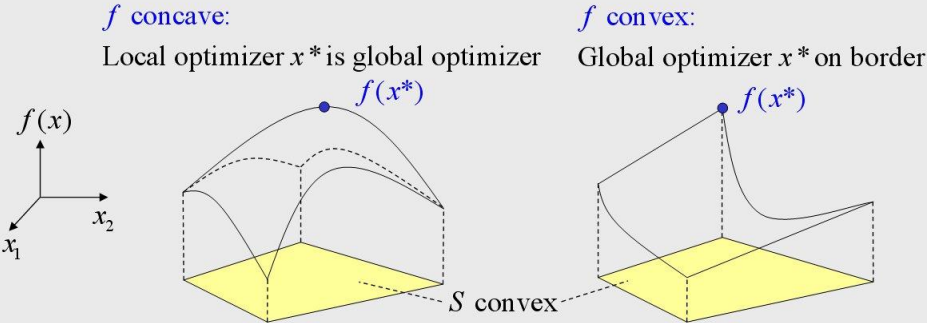
\includegraphics[width=8cm]{./Content/OptMathModels/ConvexBorderSolution}
      \\
    Lineare Funktion
      & Für den Fall einer linearen Funktion $f$ über einer konvexen, begrenzten, abgeschlossenen Menge $S$ gilt, dass jede lokale Optimallösung global optimal ist und sich am Rand von $S$ befindet!\\
  \end{tabularx}
  
\subsection{Mengenlehre}  

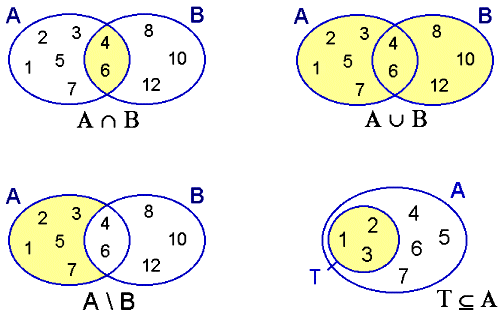
\includegraphics[width=7cm]{./Content/OptMathModels/Mengenlehre}

  
\subsection{Typen von Optimierungsmodellen und -methoden \skript{46}}

\textbf{Optimisierungsmodelle:}
\begin{itemize}
  \item Constrained vs. Unconstrained
  \item Global vs. Lokal
  \item Differenzierbar vs. Nicht-Differenzierbar
  \item Diskret vs. Kontinuierlich
  \item Konvex vs. Nicht-Konvex
  \item Linear vs. Nichtlinear
\end{itemize}

\textbf{Optimisierungsmethoden:}
\begin{itemize}
  \item Exakt vs. Heuristisch
  \item Generell vs. Problemspezifisch
\end{itemize}

Typen von Heuristiken:
\begin{itemize}
  \item Konstruktiv
  \item Verbessernde Heuristiken
  \begin{itemize}
    \item Lokale Suche (\textit{local search})
    \item generelle Meta-Heuristiken (\textit{general meta heuristics})
  \end{itemize}
\end{itemize}

\clearpage
\section{Lineare Programmierung \skript{49}}

\subsection{Problemformulierung}
  \subsubsection{Notationen}
    \begin{tabular}{p{6cm} l}
      Variablen (Spalten) & $x \in \mathbb{R}^n$; $I = \{1, ..., m\}$ \\
      Constraints ((Un-)gleichungen; Zeilen) & $a^k$; $J = \{1, ..., n\}$ \\
      Matrix & $A \in \mathbb{R}^{m \times n}$
    \end{tabular}
    
    \begin{tabularx}{\textwidth}{|X|p{4.5cm}|p{5.5cm}|p{2cm}|}
    \hline
      Lineares Problem (Beispiel U4-1)
        & $\max x_1 + 3 x_2 + 2x_3$
        & $x_2 + x_3 \leq 2$ \newline 
          $x_1 - 2x_2 \leq -2$
        & $x_1, x_2, x_3 \geq 0$\\
      \hline
      \hline
      Zeilennotation
        & $\max c x$ \newline
        $c$ = Zeilenvektor $1 \times n$\newline
        $x$ = Spaltenvektor $n \times 1$
        & $a^i x \leq b_i, \;i=1,...,m$ \newline
        $a^i$ = Zeilenvektor $1 \times n$\newline
        $x$ = Spaltenvektor $n \times 1$
        & $x \geq 0$\\
      Beispiel
        & $\max [1, 3, 2]
          \begin{bmatrix}
            x_1\\x_2\\x_3
          \end{bmatrix}$
        & $a^1: \; [0,1,1]
          \begin{bmatrix}
            x_1\\x_2\\x_3
          \end{bmatrix} \leq 2$\newline
          $a^2: \; [1,-2,0]
          \begin{bmatrix}
            x_1\\x_2\\x_3
          \end{bmatrix} \leq -2$
        & $x \geq 0$
        \\
      \hline
      Spaltennotation
        & $\max c x$ \newline
        $c$ = Zeilenvektor $1 \times n$\newline
        $x$ = Spaltenvektor $n \times 1$
        & $\sum\limits_{j=1}^{n}A_j x_j \leq b$ \newline
        $A_j$ = Spaltenvektor $n \times 1$ \newline 
        $b$ = Spaltenvektor $n \times 1$
        & $x \geq 0$
        \\
      Beispiel
        & $\max [1,3,2]
          \begin{bmatrix}
            x_1\\x_2\\x_3
          \end{bmatrix}$
        & $\begin{bmatrix}
            0\\1
          \end{bmatrix} x_1 + 
          \begin{bmatrix}
            1\\-2
          \end{bmatrix} x_2 + 
          \begin{bmatrix}
            1\\0
          \end{bmatrix} x_3
          \leq \begin{bmatrix}
            2 \\ -2
          \end{bmatrix}$
        &  $x \geq 0$
        \\
      \hline
      Matrixnotation
        & $\max c x$ \newline
        $c$ = Zeilenvektor $1 \times n$\newline
        $x$ = Spaltenvektor $n \times 1$
        & $A x \leq b$ \newline
        $A$ = Matrix $m \times n$\newline
        $b$ = Spaltenvektor $m \times 1$
        & $x \geq 0$
        \\
      Beispiel
        & $\max [1, 3, 2]
          \begin{bmatrix}
            x_1\\x_2\\x_3
          \end{bmatrix}$
        & $\begin{bmatrix}
            0& 1 & 1\\
            1& -2 & 0
          \end{bmatrix}
          \begin{bmatrix}
            x_1\\x_2\\x_3
          \end{bmatrix}
          \leq \begin{bmatrix}
            2 \\ -2
          \end{bmatrix}$
        &  $x \geq 0$
        \\
      \hline
    \end{tabularx}


  \subsubsection{Normalformen}
    Ein lineares Programm kann in verschiedenen Formen geschrieben werden:
    
    \begin{tabularx}{\textwidth}{|l|X|}
      \hline
      Allgemeine Form & 
          max / min $cx$ \newline
          $a^ix \leq b_i,$ \newline
          $a^ix = b_i,$ \newline
          $a^ix \geq b_i,$ \newline
          $x_j \geq 0,$ \newline
          $x_j \text{ frei},$ \newline
          $x_j \leq 0$
          \\
      \hline
      Kanonische Form & 
          max $cx$ \newline
          $a^ix \leq b_i,$ \newline
          $x_j \geq 0$ \newline
          \em oder \em\newline
          min $cx$ \newline
          $a^ix \geq b_i,$ \newline
          $x_j \geq 0$
         \\
      \hline
      Standardform & 
        max / min $cx$ \newline
        $a^ix = b_i,$ \newline
        $x_j \geq 0$
        \\
      \hline
      Ungleichungsform & 
        max $cx$ \newline
        $a^ix \leq b_i,$ \newline
        \em oder \em \newline
        min $cx$ \newline
        $a^ix \geq b_i,$
        \\
      \hline
    \end{tabularx}

    Zusätzlich wird zwischen Maximierungs- und Minimierungsproblemen unterschieden.
    
  \subsubsection{Umformulierungen \skript{51}}
    \label{sec:linprog_umwandlungen}
   	Achtung: Freie Variable ($x_j = $ frei) und nicht positive ($x_i \leq 0$) als allererstes in allen Formulierungen (Funktion, Bedingungen) ersetzen!
    	
    \begin{tabularx}{\linewidth}{p{0.3\linewidth}X}
      \textbf{Non-positive to non-negative variables:} & \(x_j \leq 0 \qquad \rightsquigarrow \qquad x_j := -\overline{x_j}, \quad \overline{x_j} \geq 0\)\\
      \textbf{Free to non-negative variables:} & \(x_j \text{ frei} \qquad \rightsquigarrow \qquad x_j := x_j^+ - x_j^-, \quad x_j^+, x_j^- \geq 0\)\\
      \textbf{Equations to inequalities:} & \(a^i x = b_i \qquad \rightsquigarrow \qquad a^i x \leq b_i, \quad a^i x \geq b_i\)\\
      \textbf{Inequalities ''\(\leq\)'' to inequalities ''\(\geq\)'' (and vice versa):} & \(a^i x \leq b_i \qquad \rightsquigarrow \qquad -a^i x \geq -b_i$ bzw. $a^i x \geq b_i \qquad \rightsquigarrow \qquad -a^i x \leq -b_i\)\\
      \textbf{Inequalities to equations:} & \(a^i x \leq b_i \qquad \rightsquigarrow \qquad a^i x + x_i^s = b_i, \quad x_i^s \geq 0\) bzw. \(a^i x \geq b_i \qquad \rightsquigarrow \qquad a^i x - x_i^s = b_i, \quad x_i^s \geq 0\)\\
    \end{tabularx}
    \(\min \{cx\} \qquad \rightsquigarrow \qquad \max \{-cx\} \qquad \qquad\) bzw. \(\qquad \max \{cx\} \qquad \rightsquigarrow \qquad \min \{-cx\}\)\\
    \(\min \{cx: x \in P\} = \textcolor{red}{-} \max \{-cx: x \in P\} \quad\) bzw. \(\quad \max \{cx: x \in P\} = \textcolor{red}{-} \min \{-cx: x \in P\}\) (für Funktionsevaluation)\\
  	
	%\todo{Beispiel Umformung von und in Standardform (Bild mit entstehender Projektion ersichtlich)}
	
	Beispiel Umformung von Ungleichung in Gleichung: $x_1 + 2x_2 + 4x_3 \geq 12 \quad \rightsquigarrow \quad x_1 + 2x_2 + 4x_3 - x_1^s = 12, \; x_1^s \geq 0$
	
	Beispiel Umformung von Gleichung in Ungleichung: $x_1 - x_2 + x_3 = 2 \quad \rightsquigarrow \quad x_1 -x_2 + x_3 \leq 2\, \wedge \, x_1 - x_2 + x_3 \geq 2$
	
	\subsubsection{Rang einer Matrix / Eckpunkte einer Matrix}
	  $\rank(A)$ = Maximal Anzahl linear unabhängiger Spalten. Eine Matrix hat Eckpunkte, wenn sie vollen Spaltenrang hat. Dies ist erfüllt, wenn das Gleichungssystem $\lambda_1 \begin{bmatrix}
   	  a_{11}\\a_{21}\\ \vdots
 	  \end{bmatrix} + 
 	  \lambda_2\begin{bmatrix}
   	  a_{12}\\a_{22}\\ \vdots
 	  \end{bmatrix} ...
 	  = \underline{0} = \begin{bmatrix}
 	     	  0\\0\\ \vdots
 	  \end{bmatrix}$ nur für $\lambda_1 = \lambda_2 = ... = 0$ erfüllt wird.
 	  
 	\subsubsection{Graphische Darstellung}
 	  Achtung: Minimierung: $-c$ Richtung! Maximierung: $+c$ Richtung!\\
 	  
 	\begin{minipage}{6.2cm}
 		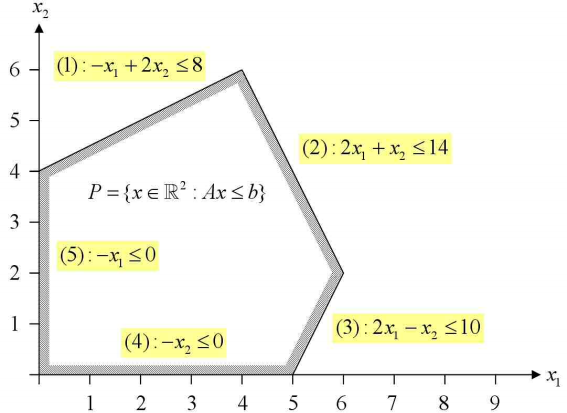
\includegraphics[width=6.3cm]{./Content/LinProg/Hyperplanes}
 	\end{minipage}
 	\begin{minipage}{6.8cm}
 	 	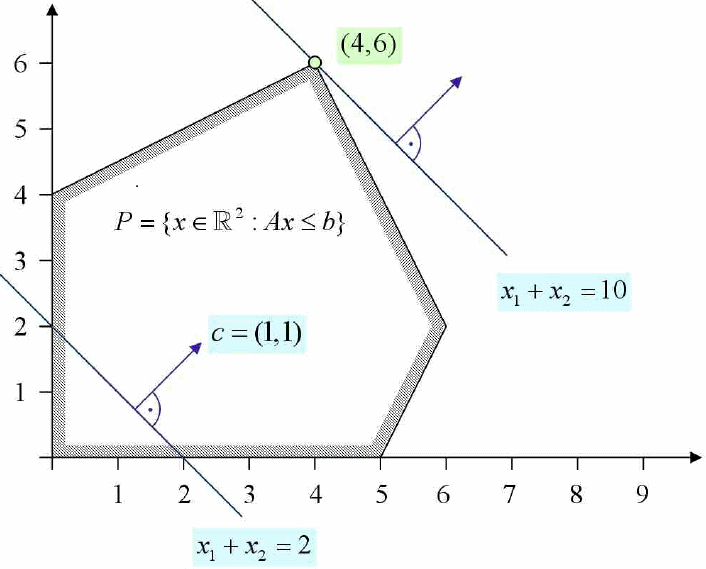
\includegraphics[width=6.3cm]{./Content/LinProg/SolveGraph}
 	\end{minipage}
 	\begin{minipage}{5.9cm}
 	 	 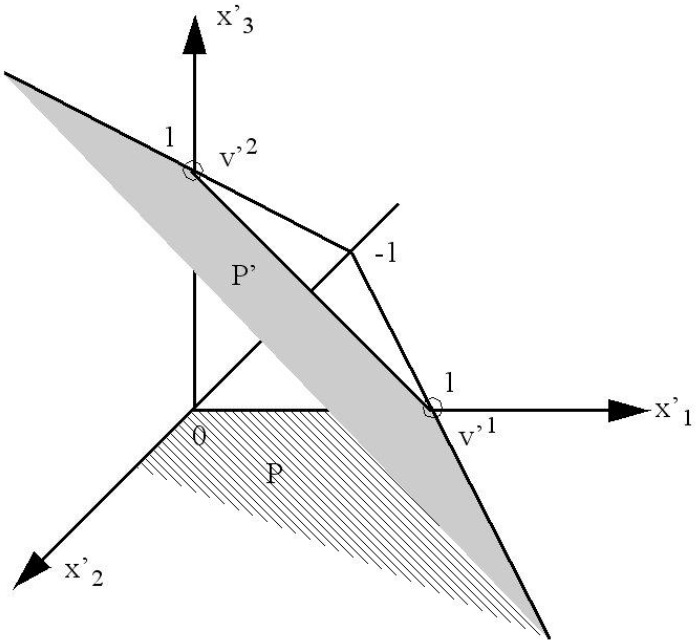
\includegraphics[width=6.3cm]{./Content/LinProg/Koordinatensystem}
 	\end{minipage}
 	
 	  
  \subsubsection{Hyperebenen}
    Die definierenden Hyperebenen sind die Gleichungen, welche den Optimierungsbereich abgrenzen, d.h. pro Gleichung oder Bedingung (in bspw. $Ax \leq b$) entsteht eine Hyperebene. Die Notation lautet z.B. $H_1 = \{x \in \mathbb{R}^3: x_1 + x_2 + x_3 = 2\}$. Die maximale Anzahl von Hyperebenen ist gleich der Anzahl Gleichungen.
    
  \subsubsection{Basisauswahl}
    Es sind bei $n$ Dimensionen $n$ Zeilen auszuwählen. Dabei sollen doppelte Gleichungen von Anfang an ignoriert werden.
    Es sind bis zu $\binom{m}{n}$ Auswahlmöglichkeiten vorhanden ($m$ = \#Gleichungen, $n$ = \#Variablen).
    
    \[ A \in \mathbb{R}^{m\times n} \qquad P = \{ x \in \mathbb{R}^{m\times n} : A x \leq b \} \qquad \qquad \text{Basisauswahl: }B\subseteq \{1,2,...,n\} \qquad  A_B : \text{ Basis von }A \]
    
    \textbf{Bsp.:}
    \[  A=
    	\begin{bmatrix}
    		\textcolor{red}{1} & \textcolor{red}{0} \\
    		1 & 1 \\
    		\textcolor{red}{-1} & \textcolor{red}{1} \\
    		0 & -1
    	\end{bmatrix}
    	\qquad
    	B=\{1,3\} \longrightarrow A_B = 
    	\begin{bmatrix}
 	    		1 & 0 \\
 	    		-1 & 1
    	 \end{bmatrix}
    \]
    
    
  \subsubsection{Basislösung}
  	Berechnung der Basislösung von $P = \{ x \in \mathbb{R}^{m\times n} : A x \leq b \}$ und $B\subseteq \{1,2,...,n\}$:
  	\[ x = A_B^{-1} \cdot b_B \]
  	Die \textbf{Basislösung} ist \textbf{gültig} wenn $\mathbf{x \in P}$ und entspricht dann einem Eckpunkt $v=x$ des Polyeders $P$!!!!
    Um die Basislösung zu bestimmen muss $\mathbf{\det(A_B)\neq 0}$ sein (linear unabhängig).
    
%    Aus Übung 3-2e: $B_1 = \{1,3,5\}:$\\
%    $x_{B_1} = \begin{bmatrix}
%      1 & 1 & 1\\
%      0 & 1 & 0\\
%      -1 & 0 & 0\\
%    \end{bmatrix}^{-1} \begin{bmatrix}
%      2\\ 1 \\0
%    \end{bmatrix} \underbrace{=}_{\text{Zeilen müssen linear unabhängig sein!}} \begin{bmatrix}
%      0\\ 1 \\ 1
%    \end{bmatrix} \underbrace{=}_{\text{Wenn Eckpunkt, dann ist Basisauswahl zulässig}} v_k$
    
%\subsection{Simplex Algorithmus \skript{56}}
%  Siehe auch Übungen 4, Aufgabe 3.
%  
%  \begin{aufzaehlung}
%    \item Als Maximierungsproblem mit $\leq$ Bedingungen umformulieren
%    \item In Matrixschreibweise umschreiben (Matrix $A$ mit einer Variable pro Spalte und einer 
%      Bedingung pro Zeile, $b$ als Spaltenvektor mit einer Bedingung pro Zeile, $c$ als 
%      Zeilenvektor mit den Koeffizienten der Maximierung)
%    \item Basisauswahl $B$ (Menge) bestimmen indem an jeweiligem Eckpunkt $v$ (Spaltenvektor) die betroffenen Bedingungen
%          festgestellt werden.
%    \item Iterationen mit jeweiligem Eckpunkt (Bsp. Bild von $v=(2,4)^T$):
%        
%        \begin{center}
%        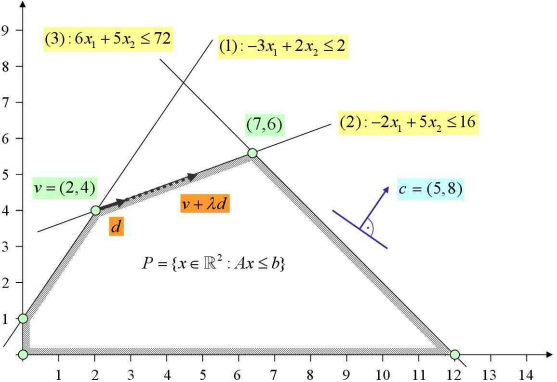
\includegraphics[width=9cm]{./Content/LinProg/simplex}
%        \end{center}
%  
%        \begin{aufzaehlung}
%          \item Basisinverse $\bar{A} = A_B^{-1}$ und evtl. zur Kontrolle Basislösung (= Eckpunkt) $v = \bar{A} b_B$ berechnen
%          \item Reduzierte Kosten berechnen: $u = c \bar{A}$
%          \item Wenn $u \geq 0$, dann Stopp!
%          \item ($u \ngeq 0$). Wähle Spalte $j \in B$ in $u$ ($u_j < 0$) und berechne daraus 
%            $d = - \bar{A}_j$, wobei $j$ in $\bar{A}_j$ die Spalte indiziert. $d$ entspricht der 
%            Richtung, in der vom Eckpunkt weitergesucht wird.
%          \item Stelle die Ungleichung $A v + \lambda A d \leq b$ mit $\lambda \in \mathbb{R}_0$ auf.
%          \item Wenn $Ad \leq 0$, dann ist die grösste Zahl $\lambda$ welche obige Ungleichung erfüllt
%            $\lambda^* = \infty$ und es muss gestoppt werden.
%          \item ($0 \leq \lambda^* < \infty$). Berechne 
%            $\lambda^* = \min \left\{ \frac{b_k - (Av)_k}{(Ad)_k} : k \in \{1,\ldots,m\}, (Ad)_k > 0 \right\}$,
%            d.h. beachte nur Zeilen, wo $(Ad)_k > 0$ ist und berechne den Bruch; der kleinste Index $k$ 
%            ist gesucht.
%          \item Bilde neue zulässige Basisauswahl $B' = B - \{j\} \cup \{k\}$, wobei $j$ in die 
%            Indizierung von der Basismatrix $A_B$ in der ursprünglichen $A$-Matrix zurückberechnet
%            werden soll.
%          \item Neuer Eckpunkt: $v' = v + \lambda^* d$
%          \item Nächste Iteration mit $B = B'$ und $v = v'$ \ldots
%        \end{aufzaehlung}
%      \item Die Optimallösung: $f(v) = cv$
%  \end{aufzaehlung}
%  
%\todo{Beispiel mit Zahlen!!!!!}

\

\section{Simplex-Algorithmus}

\begin{enumerate}
\item \textbf{Vorbereitung:}
	\begin{itemize}
	\item \textbf{Lineares Programm (LP) in Ungleichungsform bringen:}\\
	$\boxed{\max\{\mathbf{c} \mathbf{x}, \mathbf{x}\in\mathbb{R}^n :\mathbf{Ax}\leq \mathbf{b}\}\\}$\quad(Alle Nebenbedingungen mit $\leq$ formulieren; $\mathbf{c}$ ist ein Zeilenvektor)
	\item \textbf{Erste zulässige Basisauswahl} $B=\begin{Bmatrix}\ldots\end{Bmatrix}$, für beliebigen Eckpunkt (Vertex) des Polyeders, \textbf{treffen:}\\
	Bei Vorgabe einer Ecke bilden die Ungleichungen welche diese Ecke definieren, die erste Basis.
	\end{itemize}
	
	\vspace{0.3cm}
	
\item \textbf{Algorithmus:}
	\begin{enumerate}
	\item \textbf{Basis bestimmen: } $\boxed{\mathbf{A}_B=\{\mathbf{A}\}_{B}}$\quad und \quad $\boxed{\mathbf{b}_{B}=\{\mathbf{b}\}_{B}}$\quad ($B_i$-te Zeilen aus \textbf{A} und \textbf{b} auswählen)\\
	\item Berechnung der \textbf{Basis-Inversen: }$\boxed{\overline{\mathbf{A}}=\mathbf{A}_B^{-1}}$\quad und der dazugehörigen \textbf{Basis-Lösung: }$\boxed{\mathbf{v}=\mathbf{\overline{A}}\cdot\mathbf{b}_B}$\\
	\item Berechnung der \textbf{''reduzierten Kosten''}: $\boxed{\mathbf{u}=\mathbf{c\overline{A}}}$
	\begin{itemize}
		\item $u_i<0$: Den ''negativsten'' Wert $u_j$ von $\mathbf{u}$ und die dazugehörige Spalte $\mathbf{\overline{a}}_j$ von $\mathbf{\overline{A}}$ bestimmen.\\
		(Wenn die $j$-te Zahl in $u$ der ''negativsten'' Zahl entspricht so ist die $j$-te Spalte in $\mathbf{\overline{A}}$ die dazugehörige Spalte). Behalte $j$ als Index der ursprünglichen Matrix $\mathbf{A}$!
		\item $u_i\geq 0$: Wenn $\mathbf{u}$ keine negativen Werte aufweist, wurde das Maximum der Zielfunktion gefunden:\\
		\textbf{Argument der Maximalstelle:} $\boxed{\mathbf{x^*}=\mathbf{v}}$\\
		\textbf{Maximalstelle:} 
		$\boxed{f(\mathbf{x^*})=\left\{
		  \begin{array}{ll}
		    \mathbf{c}\cdot\mathbf{v} & \text{Wenn anfängliches Problem eine Maximierung war}\\
		    -\mathbf{c}\cdot\mathbf{v}& \text{Wenn anfängliches Problem eine Minimierung war}
		  \end{array}
		\right.}$
	\end{itemize}
	\item \textbf{Richtungsvektor} für Bewegung auf Kante: $\boxed{\mathbf{d}=-\mathbf{\overline{A}}_j}$
	\item \textbf{Bewegung in Richtung von} $\mathbf{d}$ solange \textbf{alle} Nebenbedingungen erfüllt.\\
	
	$\boxed{\mathbf{A}(\mathbf{v}+\lambda\cdot \mathbf{d})\leq \mathbf{b}}\quad\Rightarrow\quad\lambda^*$\quad($\lambda^*$ ist der Maximalwert von $\lambda$ welcher alle Nebenbedingungen noch erfüllt.)\\
		
	Berechnung von $k$: $\lambda^* = \min\limits_k \left\{ \frac{b_i-\mathbf{a}^i\mathbf{v}}{\mathbf{a}^i\mathbf{d}}: i \in I, \mathbf{a}^i\mathbf{d} > 0\right\}$
		
	\begin{itemize}
		\item $0\leq\lambda^*<\infty$\qquad \textbf{Weiter mit (f):} Zielfunktion in Richtung $\mathbf{d}$ durch Bedingung $k$ beschränkt
		\item $\lambda^*\rightarrow\infty$\qquad\quad~ \textbf{Abbruch:} Zielfunktion wächst unbeschränkt in Richtung von $\mathbf{d}$
	\end{itemize}
	\item \textbf{Basistausch:} $B'(j)=k$ bzw. $B' = B - (\{j\} \cup \{k\})$\qquad $\boxed{\mathbf{v'}=\mathbf{v}+\lambda^*\cdot \mathbf{d}}$\quad (Die Basis an $j$-ter Stelle in B wird durch $k$ ersetzt)\\
	
	\textbf{Setze} $\boxed{B:=B'}$,\quad $\boxed{\mathbf{v}:=\mathbf{v'}}$ und \textbf{beginne bei Punkt (a)}
	\end{enumerate}
\end{enumerate}

\subsection{Beispiel:}
Das unten stehende LP-System soll mittels Simplexalgorithmus gelöst werden. Es soll im Punkt $V_0=\begin{bmatrix}0 & 1\end{bmatrix}$ begonnen werden.\\

\begin{minipage}[t]{0.66\textwidth}
	\begin{minipage}[t]{0.3\linewidth}
		\textbf{1.Durchlauf} \\
		$\max~~\{x_1-2x_2\}$\\
		$\begin{array}{ccc}
			x_1+x_2 & \leq & 2\\
			x_1 & \geq & 0\\
			x_2 & \leq & 1\\
			x_2 & \geq & -1\\
			
			
		\end{array}$
	\end{minipage}
	\hfill
	\begin{minipage}[t]{0.34\linewidth}
		\textbf{In Ungleichungsform:} \\
		$\max~~\{x_1-2x_2\}$\\
		$\begin{array}{ccc}
			x_1+x_2 & \leq & 2\\
			-x_1 & \leq & 0\\
			x_2 & \leq & 1\\
			-x_2 & \leq & 1\\
			
		\end{array}$
	\end{minipage}
	\hfill
	\begin{minipage}[t]{0.34\linewidth}
	\textbf{Matrizenschreibweise:}\\
	$c=\begin{bmatrix}
	1&-2
	\end{bmatrix}$\\
	$A=\begin{bmatrix}
	1  &  1 \\
	-1 &  0 \\
	 0 &  1 \\
	 0 & -1 
	\end{bmatrix}\quad 
	b=\begin{bmatrix}
	2\\
	0\\
	1\\
	1
	\end{bmatrix}$
	\end{minipage}\\
	\\
	
Die erste zulässige Basis: $B=\begin{Bmatrix}2&3\end{Bmatrix}\quad\Rightarrow\quad \mathbf{A_B}=\begin{bmatrix}-1&0\\0&1\end{bmatrix},\quad \mathbf{b_B}=\begin{bmatrix}0\\1\end{bmatrix}$

\subsubsection{Algorithmus}
 
\textbf{1.Durchlauf}
\begin{itemize}
\item[(a)] $\mathbf{A_B}=\{\mathbf{A}\}_{\mathbf{B}}=\begin{bmatrix}-1&0\\0&1\end{bmatrix}$\qquad $\mathbf{b}_\mathbf{B}=\{\mathbf{b}\}_{\mathbf{B}}=\begin{bmatrix}0\\1\end{bmatrix}$
\item[(b)] $\overline{\mathbf{A}}=\mathbf{A_B}^{-1}=\begin{bmatrix}-1&0\\0&1\end{bmatrix}^{-1}=\begin{bmatrix}-1&0\\0&1\end{bmatrix}\qquad
\mathbf{v}=\mathbf{\overline{A}}\cdot\mathbf{b_B}=\begin{bmatrix}0\\1\end{bmatrix}$


\end{itemize}
\end{minipage}
\hfill
\begin{minipage}[t]{0.30\textwidth}
\textbf{Zeichnung:}\\
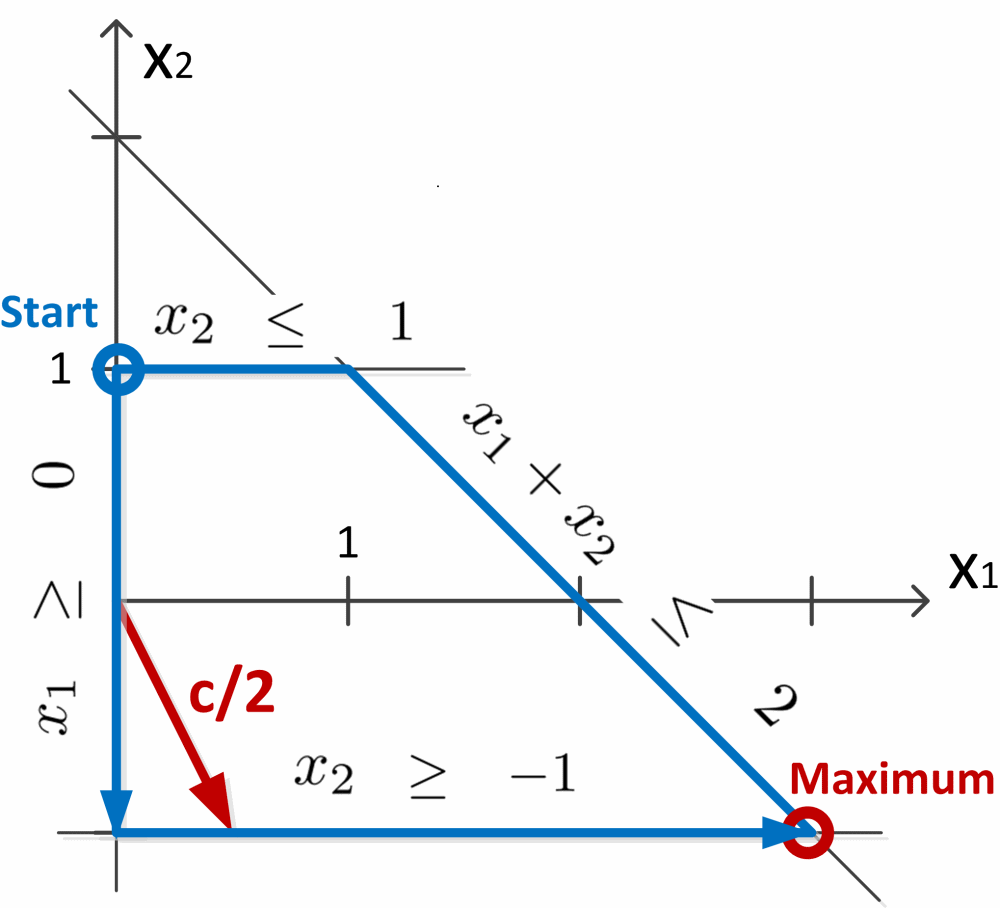
\includegraphics[width=\linewidth]{Content/Simplex/Polyeder.png} 
\end{minipage}
\begin{itemize}
	\item[(c)] $\mathbf{u}=\mathbf{c\overline{A}}=\begin{bmatrix}1&-2\end{bmatrix}\cdot\begin{bmatrix}-1&0\\0&1\end{bmatrix}=\begin{bmatrix}-1&-2\end{bmatrix}\quad\Rightarrow\quad \mathbf{\overline{a}}_j=\begin{bmatrix}0\\1\end{bmatrix}\qquad j=2$
	\item[(d)] $\mathbf{d}=-\mathbf{\overline{a}}_j=\begin{bmatrix}0\\-1\end{bmatrix}$ 
	\item[(e)] $\mathbf{A}(\mathbf{v}+\lambda\cdot \mathbf{d})\leq \mathbf{b}\quad\Rightarrow\quad\begin{bmatrix}
		1  &  1 \\
		-1 &  0 \\
		 0 &  1 \\
		 0 & -1 
		\end{bmatrix}\cdot\left(\begin{bmatrix}0\\1\end{bmatrix}+\lambda\cdot\begin{bmatrix}0\\-1\end{bmatrix}\right)\leq \begin{bmatrix}
			2\\
			0\\
			1\\
			1
			\end{bmatrix}\quad\Rightarrow\quad\begin{bmatrix}1\\0\\1\\-1\end{bmatrix}+
			\begin{bmatrix}-\lambda\\0\\-\lambda\\\lambda\end{bmatrix}\leq\begin{bmatrix}2\\0\\1\\1\end{bmatrix}\quad\Rightarrow\quad\lambda^*=2\qquad k=4$
	\item[(f)] $B'(j)=k\quad\Rightarrow\quad B'=\begin{Bmatrix}2&4\end{Bmatrix}\qquad \mathbf{v'}=\mathbf{v}+\lambda^*\cdot \mathbf{d}=\begin{bmatrix}0\\1\end{bmatrix}+2\cdot\begin{bmatrix}0\\-1\end{bmatrix}=\begin{bmatrix}0\\-1\end{bmatrix}$
\end{itemize}

\vspace{0.5cm}
\textbf{2.Durchlauf}
\begin{itemize}
	\item[(a)] $\mathbf{A_B}=\{\mathbf{A}\}_{\mathbf{B}}=\begin{bmatrix}-1&0\\0&-1\end{bmatrix}$\qquad $\mathbf{b}_\mathbf{B}=\{\mathbf{b}\}_{\mathbf{B}}=\begin{bmatrix}0\\1\end{bmatrix}$
	\item[(b)] $\overline{\mathbf{A}}=\mathbf{A_B}^{-1}=\begin{bmatrix}-1&0\\0&-1\end{bmatrix}^{-1}=\begin{bmatrix}-1&0\\0&-1\end{bmatrix}\qquad
	\mathbf{v}=\mathbf{\overline{A}}\cdot\mathbf{b_B}=\begin{bmatrix}0\\-1\end{bmatrix}$
	\item[(c)] $\mathbf{u}=\mathbf{c\overline{A}}=\begin{bmatrix}1&-2\end{bmatrix}\cdot\begin{bmatrix}-1&0\\0&-1\end{bmatrix}=\begin{bmatrix}-1&2\end{bmatrix}\quad\Rightarrow\quad \mathbf{\overline{a}}_j=\begin{bmatrix}-1\\0\end{bmatrix}\qquad j=1$
	\item[(d)] $\mathbf{d}=-\mathbf{\overline{a}}_j=\begin{bmatrix}1\\0\end{bmatrix}$ 
	\item[(e)] $\mathbf{A}(\mathbf{v}+\lambda\cdot \mathbf{d})\leq \mathbf{b}\quad\Rightarrow\quad\begin{bmatrix}
		1  &  1 \\
		-1 &  0 \\
		 0 &  1 \\
		 0 & -1 
		\end{bmatrix}\cdot\left(\begin{bmatrix}0\\-1\end{bmatrix}+\lambda\cdot\begin{bmatrix}1\\0\end{bmatrix}\right)\leq \begin{bmatrix}
			2\\
			0\\
			1\\
			1
			\end{bmatrix}\quad\Rightarrow\quad\begin{bmatrix}-1\\0\\-1\\1\end{bmatrix}+
			\begin{bmatrix}\lambda\\-\lambda\\0\\0\end{bmatrix}\leq\begin{bmatrix}2\\0\\1\\1\end{bmatrix}\quad\Rightarrow\quad\lambda^*=3\qquad k=1$
	\item[(f)] $B'(j)=k\quad\Rightarrow\quad B'=\begin{Bmatrix}1&4\end{Bmatrix}\qquad \mathbf{v'}=\mathbf{v}+\lambda^*\cdot \mathbf{d}=\begin{bmatrix}0\\-1\end{bmatrix}+3\cdot\begin{bmatrix}1\\0\end{bmatrix}=\begin{bmatrix}3\\-1\end{bmatrix}$
\end{itemize}

\vspace{0.5cm}
\textbf{3.Durchlauf}
\begin{itemize}
	\item[(a)] $\mathbf{A_B}=\{\mathbf{A}\}_{\mathbf{B}}=\begin{bmatrix}1&1\\0&-1\end{bmatrix}$\qquad $\mathbf{b}_\mathbf{B}=\{\mathbf{b}\}_{\mathbf{B}}=\begin{bmatrix}2\\1\end{bmatrix}$
	\item[(b)] $\overline{\mathbf{A}}=\mathbf{A_B}^{-1}=\begin{bmatrix}1&1\\0&-1\end{bmatrix}^{-1}=\begin{bmatrix}1&1\\0&-1\end{bmatrix}\qquad
	\mathbf{v}=\mathbf{\overline{A}}\cdot\mathbf{b_B}=\begin{bmatrix}3\\-1\end{bmatrix}$
	\item[(c)] $\mathbf{u}=\mathbf{c\overline{A}}=\begin{bmatrix}1&-2\end{bmatrix}\cdot\begin{bmatrix}1&1\\0&-1\end{bmatrix}=\begin{bmatrix}1&3\end{bmatrix}$\\
	\textbf{Argument der Maximalstelle:} $\mathbf{x^*}=\mathbf{v}=\begin{bmatrix}3\\-1\end{bmatrix}$\qquad \textbf{Maximalstelle:} $f(\mathbf{x^*})=\mathbf{c}\cdot\mathbf{v}=\begin{bmatrix}1&-2\end{bmatrix}\cdot \begin{bmatrix}3\\-1\end{bmatrix}=5$
\end{itemize}







\section{Ganzzahlig-lineare Programmierung \skript{63}}
  \begin{minipage}{7cm}
    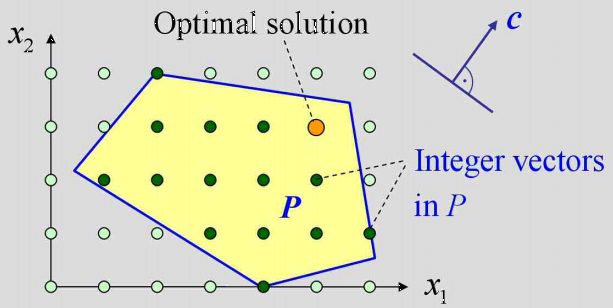
\includegraphics[width=7cm]{./Content/IntProg/intprog}
  \end{minipage}
  \begin{minipage}{12cm}
	  Als zusätzliche Nebenbedingung zu LP dürfen Variablen nur ganzzahlig (integer, ILP) sein, das macht das Problem einiges komplizierter.
	  Konkret sind LP polynomial lösbar, während ILP NP-vollständig (NP-complete) sind.
	    
  	\subsection{Relaxationen}
  		Um Schranken (obere/untere) zu berechnen, kann der \em Lösungsraum
  		vergrössert \em werden (Relaxationen). Beispiel: Der höchste Berg in
  		Tibet ist höchstens so gross wie der höchste Berg in China (China
  		$\rightarrow$ grösserer Lösungsraum als Tibet). In ILP wird \em
  		LP-Relaxation \em verwendet, d.h. die Ganzzahligkeitsforderung wird
  		fallen gelassen.
	\end{minipage}
  
		

\subsection{Branch-and-Bound Verfahren \skript{68}}
	\begin{minipage}{8cm}
		Um die optimale Lösung zu finden, wird das Lösungsgebiet aufgeteilt und jeweils sowohl eine obere als auch eine untere Schranke der Lösung gesucht. Falls die Schranken bereits eine optimale Lösung ausschliessen (wenn bei einem anderen Ast die untere Schranke höher ist als die obere beim aktuellen), kann die Suche innerhalb dieses Astes abgebrochen werden. Man spricht von \em Pruning by Dominance\em. Optimalität ist gefunden, wenn die obere gleich der unteren Schranke ist.
		
		Details für ILP: \skript{72f.}\\
		B\&B ist geeignet für beliebige Optimierungsprobleme (inkl. nichtlineare). Die Terminierung nach endlicher Anzahl Schritten ist jedoch nur bei endlichen Lösungsräumen gewährleistet.
	\end{minipage}
	\begin{minipage}{10cm}
		Beispiel: Helikopter $\Leftrightarrow$ Sherpas.
		
		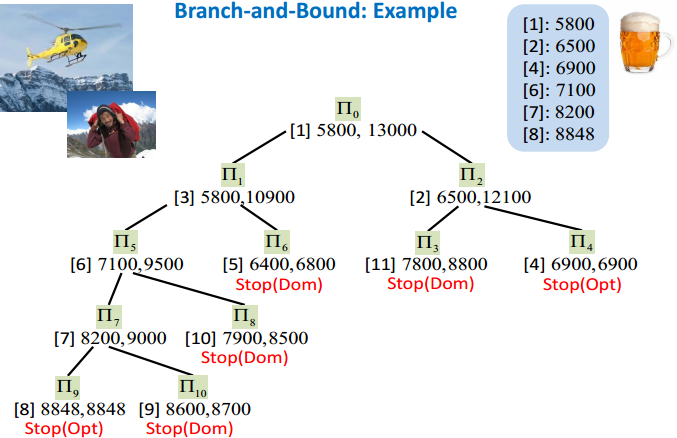
\includegraphics[width=10cm]{Content/IntProg/branch-bound}
	\end{minipage}

\subsubsection{Beispiel: ILP Übung 6.2}
\begin{minipage}{6cm}
	$\text{max } 5x_1+6x_2$\\
	$3x_1 + 6x_2 \leqslant 18$\\
	$9x_1+6x_2 \leqslant 27$\\
	$x_1,x_2 \geqslant 0, \text{integer}$\\
	
	Branching: Runden Variable mit kleinstem Index\\
	Strategie: \textit{Dept-First-Search}\\
	Jeweils aufgerundeter Knoten zuerst\\
	$[$Iteration$]$r=Knotennummer:\\
\end{minipage}
\begin{minipage}{12cm}
	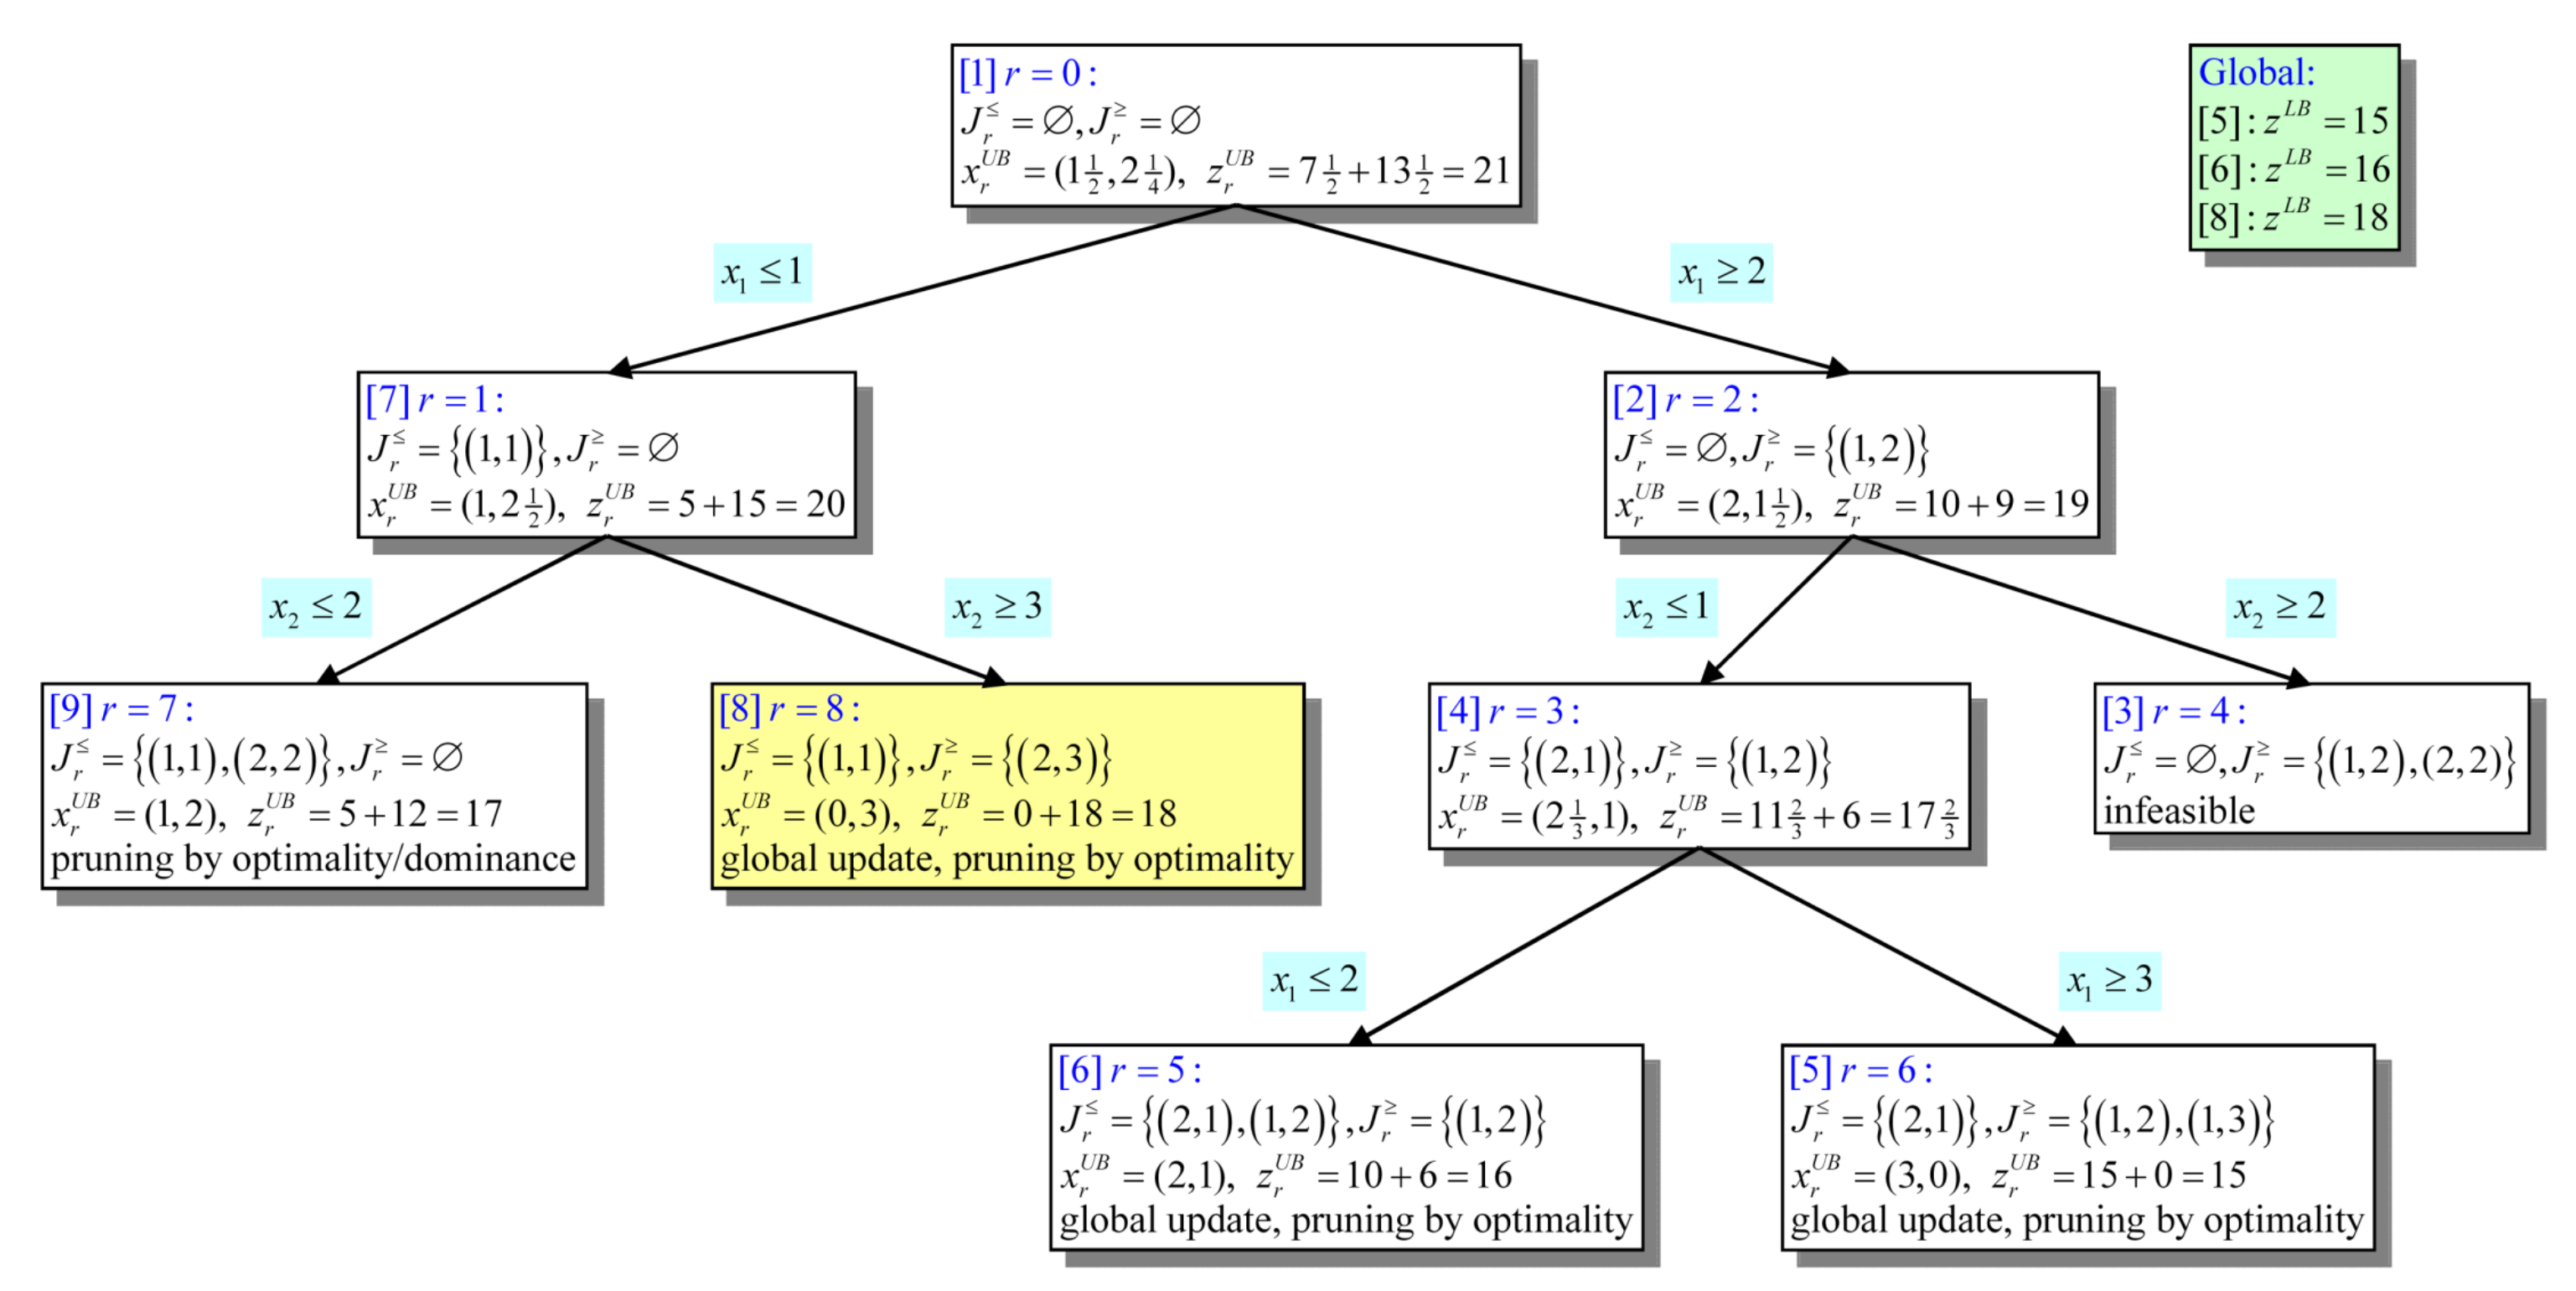
\includegraphics[width=12cm]{Content/IntProg/branch-bound-lp}
\end{minipage}

\subsubsection{Beispiel: Branch-and-bound beim Knapsack-Problem \skript{73--78}}

\textbf{Lower bound:}\\
Lower bound ist die global gespeicherte beste Item-Auswahl, die wir bis jetzt angetroffen haben und somit Kandidat für globales Optimum. (Vgl. 'Bar in Kathmandu')\\

\textbf{Upper bound:}\\
In einem beliebigen Knoten berechnet sich der upper bound wie folgt:
\begin{itemize}
	\item Items, für die im aktuellen Knoten noch keine Entscheidung getroffen wurde, sortieren nach $\frac{Wert}{Gewicht}$ ('Wertdichte').
	\item Soviele (ganze) Items einpacken wie Platz dafür vorhanden ist.
	\item Vom nächst'dichteren' einen Bruchteil einpacken, s.d. das maximale Gewicht ausgereizt ist. (LP-Relaxation)
	\item Mehr Wert kann in diesem Knoten nicht erreicht werden, somit handelt es sich um den upper bound.
	\item Wenn der upper bound kleiner ist, als was wir (global gespeichert) schon erreicht haben, können wir abbrechen. (\em pruning by dominance\em)
\end{itemize}

\textbf{Heuristische Lösungssuche:}\\
Packe von den noch nicht definitiv (ab)gewählten Elementen soviele (nach Wertdichte sortierte) ein, wie es dafür Platz im Rucksack hat. (ACHTUNG: Im Wurzelknoten hat es also typischerweise zu Beginn bereits mehr als ein Element im Rucksack.)\\

\textbf{Definition der Teilprobleme:}\\
Um aus einem Knoten die beiden Nachfolge-Knoten zu bilden wird wie folgt vorgegangen:
\begin{itemize}
	\item Dasjenige Element, das nur partiell Platz hatte im rechten Teilbaum definitv wählen und im linken definitiv abwählen.
	\item Die heuristische Lösungssuche neu durchführen.
\end{itemize}

\textbf{Strategie der Knotenwahl:}\\
Für die Wahl des nächsten zu expandierenden Knotens gibt es verschiedene Ansätze. Wir fahren eine Depth-first-search Strategie. Dazu expandieren wir immer den rechtesten Knoten, welcher noch nicht geprunt wurde.\\
 
\textbf{Arbeitsschritte:}
\begin{enumerate}
	\item Iterationsnummer inkrementieren und in eckigen Klammern notieren
	\item Zu expandierenden Knoten $r$ bestimmen (gemäss 'Strategie der Knotenwahl')
	\item Vorgänger-Knoten in Klammern notieren (falls vorhanden, sonst '.')
	\item Menge der definitiv abgewählten Knoten $J^0_r$ und definitiv gewählten Knoten $J^1_r$ notieren.
	\item Bitvektor-Auswahl für upper bound $x_r^{UB}=x^{LP}$ notieren (enthält Bruchteil von item)
	\item (Imaginären) Rucksackwert $z_r^{UB}=z^{LB}$ berechnen und auf pruning by dominance prüfen ($z_r^{UB}\le z^{LB}$) (bester bisher erreichter Wert kann sicher nicht erreicht werden); Falls pruning by dominance weiter mit Schritt 1.
	\item Bitvektor-Auswahl $x_r^{LB}$ notieren und zugehörigen Rucksackwert $z_r^{LB}$ berechnen
	\item Auf global update für lower bound $(z_r^{LB} > z^{LB})$ prüfen, ggf. updaten.
	\item Auf pruning by optimality $(z_r^{LB} = z^{UB})$ prüfen.
	\item Branching ausführen (Teilprobleme bilden)
	\item Weiter bei Schritt 1.
\end{enumerate}

\subsection{Schnittebenenverfahren (Cutting Planes) \skript{78}}  
	%\todo{RK: Keine Übungen dazu gefunden... ZF nötig??}
	
	Durch Linearkombination der Bedingungen, ist eine Einschränkung des Lösungsgebiets möglich. Die Multiplikatoren werden durch ''pröbeln'' gefunden. Beispiel:
	
	\begin{tabular}{p{8cm} p{4cm} p{3cm}}
		Ursprüngliche Bedingung 1 & $x_1 + 3 x_2 \leq 6$ & $| \cdot \frac{5}{8}$\\
		Ursprüngliche Bedingung 2 & $3 x_1 + x_2 \leq 6$ & $| \cdot \frac{1}{8}$  \\
		Aufsummiert: & $x_1 + 2 x_2 \leq \lfloor 4.5 \rfloor \overbrace{=}^{!} 4$ \\
	\end{tabular}

\subsubsection{Chvátal-Rang berechnen \skript{91}}
Für rationale Polytope $P$ existiert eine endliche Zahl $k$ (Chvátal-Rang): Es ist die kleinste Anzahl Anwendungen des obigen Verfahrens, die nötig ist, damit das Polytop zur ganzzahligen Hülle $P_\mathbb{Z}$ wird.




\section{Nichtlineare Optimierung}

\textbf{Satz von Schwarz:\skript{2}} $\frac{\partial^2 f(x_1, x_2)}{\partial x_1 \partial x_2} = \frac{\partial^2 f(x_1, x_2)}{\partial x_2 \partial x_1}$\\
Bei partiellen Ableitungen spielt die Reihenfolge keine Rolle. (Bedingung: Alle partiellen Ableitungen stetig.)

\begin{minipage}[t]{0.4\linewidth}
\subsection{Gradient\skript{3}}
Der Gradient zeigt immer in Richtung des steilsten Anstiegs der Funktion $f$ und steht senkrecht auf den Höhenlinien.\\


$\nabla f =\begin{bmatrix}
f_{x_1}\\
f_{x_2}\\
\vdots\\
f_{x_n}
\end{bmatrix}=\begin{bmatrix}
\partFrac{f}{x_1}\\[0.1cm]
\partFrac{f}{x_2}\\[0.1cm]
\vdots\\[0.1cm]
\partFrac{f}{x_n}
\end{bmatrix}$
\end{minipage}
\hfill
\begin{minipage}[t]{0.58\linewidth}
	\subsection{Algebraisch Extrema bestimmen}
	\textbf{Alle Ränder müssen seperat ansgeschaut werden!!!}\\
	(Randwerte einsetzen, dann in verbliebene Richtungen ableiten)\\
	
	\boxed{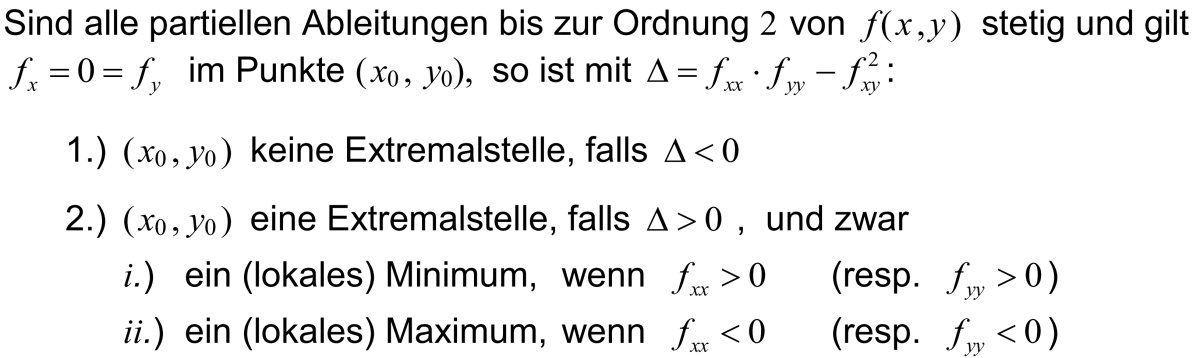
\includegraphics[width=0.9\linewidth]{./Content/NonLinearOptimization/maxMin}}\\
\end{minipage}



  \begin{minipage}[t]{8.5cm}
 \subsection{Gradientenverfahren\skript{4}}
    Von der Stelle $\vec{x}^{(i)}$ wird in Richtung des Antigradienten geschritten. 
    $$\vec{x}^{(i+1)} = \vec{x}^{(i)} - \alpha_i \nabla f(\vec{x}^{(i)})$$
\subsubsection{Eigenschaften}    
    Vorteile:
    \begin{liste}
      \item Einfach zu implementieren
      \item Findet optimale Lösung
      \item Keine gute Startnäherung nötig
    \end{liste}
    
    Nachteile:
    \begin{liste}
      \item Konvergiert langsam
      \item In der Nähe der optimalen Lösung Zick-Zack-Kurs
    \end{liste}
    
    \subsubsection{Algorithmus (zur Minimierung)}
  \end{minipage}
  \hfill
  \begin{minipage}[t]{10cm}
  	  \subsection{Differential-Rechnung}
  	  $f'(x_0)=\lim\limits_{\Delta x\rightarrow 0}
  	  \frac{f(x_0+\Delta)x-f(x_0)}{\Delta x}$\\
  	  	\begin{tabular}{llll}
  	  		Kettenregel:	& $\Bigl(f\big(g(x)\big)\Bigr)'$ &$=$ & $g'(x)\cdot f'\big(g(x)\big)$\\[0.1cm]
  	  		%oder $\frac{d f(g(x))}{dx} = f'(g(x)) \cdot g'(x)$\\[0.1cm] 
  	  		Produktregel:	& $\Bigl(f(x)\cdot g(x)\Bigr)'$ &$=$ & $f'(x)\cdot g(x) + f(x)\cdot g'(x)$\\[0.1cm]
  	  		Quotientenregel:& $\left(\frac{f(x)}{g(x)}\right)'$ &$=$ & $\frac{f'(x)g(x)-f(x)g'(x)}{g^2(x)}$\\
  	  	\end{tabular}
	  \begin{minipage}{4.5cm}
	    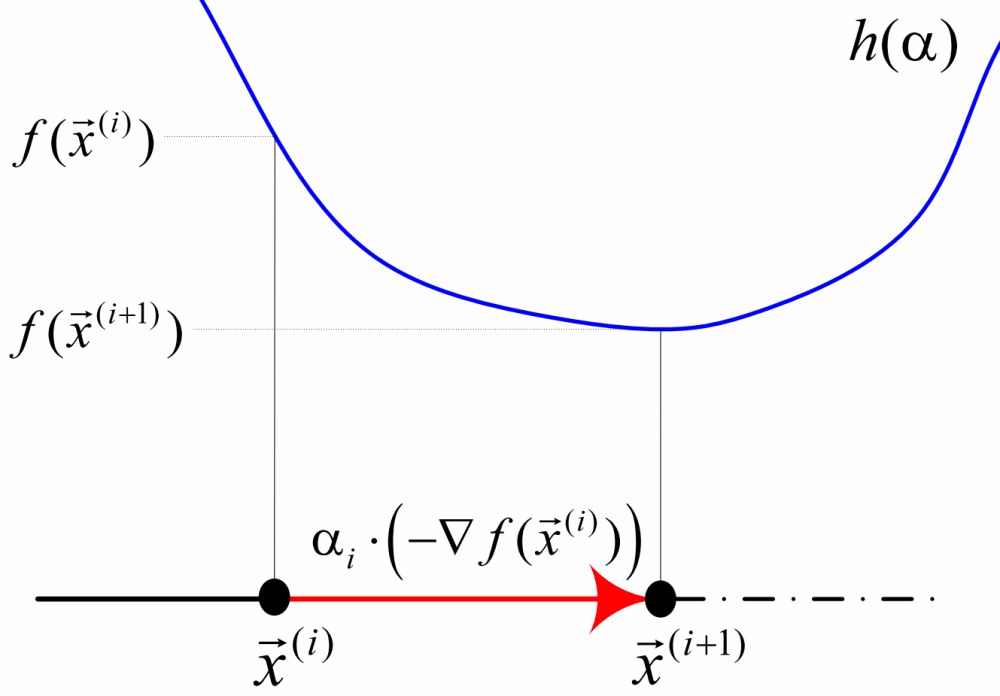
\includegraphics[width=4.5cm]{./Content/NonLinearOptimization/Gradient1D.png}
	  \end{minipage}
	  \hfill
	  \begin{minipage}{4.5cm}
	  	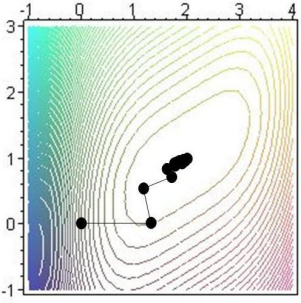
\includegraphics[width=4.5cm]{./Content/NonLinearOptimization/gradient-descent}
	  \end{minipage}
 \end{minipage}
 
 
 
 \begin{enumerate}
	\item $\beta_1=0$\quad$\beta_3=1$\qquad$h(\beta_i)=f\Bigl(\vec{x}^{(i)} - \beta_i \nabla f(\vec{x}^{(i)})\Bigr)$
	\item $while\Bigl(h(\beta_3)\geq h(\beta_1)\Bigl)\Bigl\{\beta_3=\frac{\beta_3}{2}\Bigr\}$
	\item Parabel konstruieren: $P(\beta)=A\beta^2+B\beta+C$\quad mit \quad $\beta_1=0$,\quad $\beta_2=\beta_3/2$\\
		$\begin{bmatrix}
		\beta_1^2 & \beta_1 & 1\\
		\beta_2^2 & \beta_2 & 1\\
		\beta_3^2 & \beta_3 & 1
		\end{bmatrix}\cdot\begin{bmatrix}A\\B\\C\end{bmatrix}=\begin{bmatrix}h(\beta_1)\\ h(\beta_2)\\ h(\beta_3)\\\end{bmatrix}\quad\Rightarrow\quad\begin{bmatrix}
		0 & 0 & 1\\
		\beta_3^2/4 & \beta_3/2 & 1\\
		\beta_3^2 & \beta_3 & 1
		\end{bmatrix}\cdot\begin{bmatrix}A\\B\\C\end{bmatrix}=\begin{bmatrix}h(0)\\ h(\beta_3/2)\\ h(\beta_3)\end{bmatrix}\quad\Rightarrow\quad
		\begin{bmatrix}A\\B\\C\end{bmatrix}=\begin{bmatrix}
		\frac{2h(\beta_1)-4h(\beta_2)+2h(\beta_3)}{\beta_3^2}\\[0.2cm]
		\frac{-3h(\beta_1)+4h(\beta_2)-h(\beta_3)}{\beta_3}\\[0.1cm]
		h(\beta_1)\end{bmatrix}$
  	\item $if\Bigl( \beta_3 \leq-B/2A\Bigr)\Big\{\hat{a}=\beta_3\Big\}$\\
  	$else\Big\{\hat{a}=-B/2A\Big\}$
  	\item $\vec{x}^{(i+1)} = \vec{x}^{(i)} - \hat{a}\nabla f(\vec{x}^{(i)})\quad\Rightarrow\quad $Punkt $ 1.$
  	
  	
 \end{enumerate}
 
 \subsubsection{Matlab-Implementation (nur ein Loop)}
  \begin{MatlabCode}
    % Find betas
    beta1 = 0;
    beta3 = 2; % will be divided by 2 in the loop -> start value = 1
    h_beta1 = subs(f, x, p);
    h_beta3 = 2*h_beta1; % must be higher than h_beta1 (initial)
    while h_beta1 <= h_beta3;
        beta3 = beta3 / 2;
        h_beta3 = subs(f, x, p - beta3 * gradf_numeric);
    end;
    beta2 = beta3/2;
    h_beta2 = subs(f, x, p - beta2 * gradf_numeric);

    % Parabola
    C = h_beta1;
    A = (h_beta3-2.0*h_beta2+C)/(2*beta2*beta2);
    B = (h_beta2-C)/beta2 - beta2*A;
 
    % Candidates for a
    a1 = -B / (2*A);
    a2 = beta3;
    
    % Select a
    if subs(f, x, p - beta3*gradf_numeric) <= h_beta3 
        a = a1;
    else
        a = a2;
    end
    
    
    % Calculate next step
    p = p - a * gradf_numeric;
  \end{MatlabCode}
  
\subsection{Newton-Verfahren\skript{7}}

  \begin{minipage}{13cm}
  	\textbf{Tangentengleichung:}\\
  	$t(x^{(i+1)})=f(x^{(i)})+f'(x^{(i+1)})\cdot(x^{(i)})=0\quad\Rightarrow\quad x^{(i+1)}=x^{(i)}-\frac{f(x^{(i)})}{f'(x^{(i)})}$\\
  	
  	\textbf{Bestimmung der Ableitung (numerisch):}\\
  	$f'(x^{(i)})\approx\frac{f(x^{(i)}+h)-f(x^{(i)})}{h}\qquad$ für $h<<1$\\
  	
    Anstelle des Gradienten wird eine Tangente an den Arbeitspunkt gelegt.
    $$\vec{x}^{(i+1)} = \vec{x}^{(i)} - \left(\bm H(\vec{x}^{(i)})\right)^{-1} \nabla f(\vec{x}^{(i)})$$
    mit der Hesse-Matrix
    $$\bm{H}(\vec{x})=
    \left(\frac{\partial^2f}{\partial x_i\partial x_j}(x)\right)_{i,j=1,\dots, n}=
    \begin{pmatrix}
    \frac{\partial^2 f}{\partial x_1\partial x_1}(x)&\frac{\partial^2 f}{\partial x_1\partial x_2}(x)&\cdots&\frac{\partial^2  f}{\partial x_1\partial x_n}(x)\\[0.5em]
    \frac{\partial^2 f}{\partial x_2\partial x_1}(x)&\frac{\partial^2 f}{\partial x_2\partial x_2}(x)&\cdots&\frac{\partial^2  f}{\partial x_2\partial x_n}(x)\\
    \vdots&\vdots&\ddots&\vdots\\
    \frac{\partial^2 f}{\partial x_n\partial x_1}(x)&\frac{\partial^2 f}{\partial x_n\partial x_2}(x)&\cdots&\frac{\partial^2  f}{\partial x_n\partial x_n}(x)
    \end{pmatrix}$$
    (4 Funktionsaufrufe für Diagonalelemente, sonst 3 Funktionsaufrufe)\\
    
    Vorteile:
    \begin{liste}
      \item Gutes Konvergenzverhalten
    \end{liste}
    
    Nachteile:
    \begin{liste}
      \item Hesse-Matrix benötigt zweite Ableitung (numerisch aufwendig)
      \item Inversion der Matrix skaliert schlecht ($O(n^3)$)
    \end{liste}
  \end{minipage}
  \begin{minipage}{6cm}
  	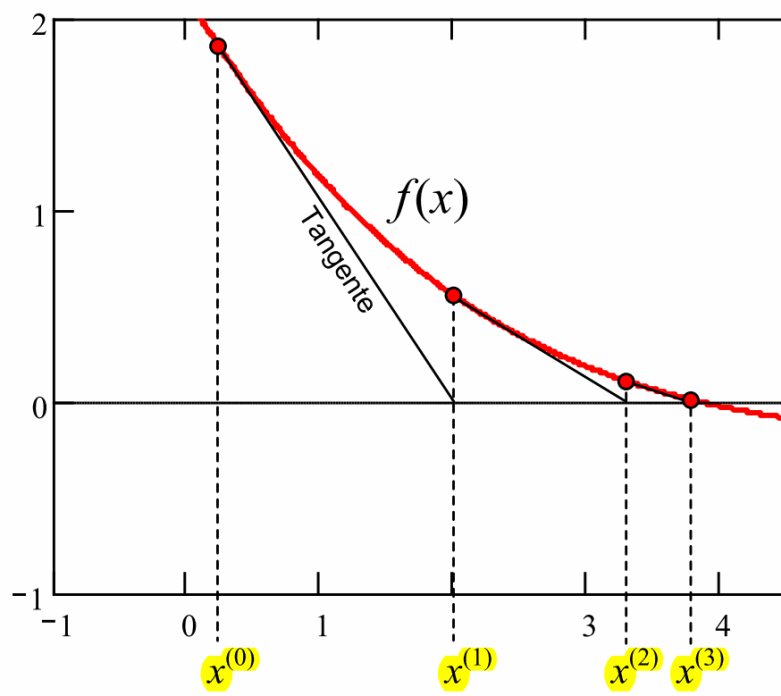
\includegraphics[width=6cm]{./Content/NonLinearOptimization/Newton1D.png}
    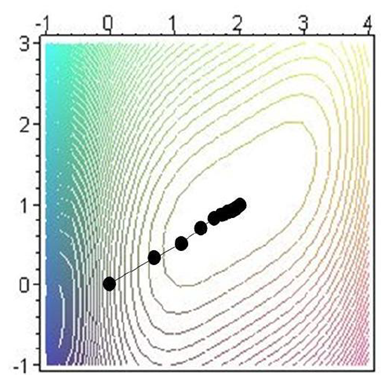
\includegraphics[width=6cm]{./Content/NonLinearOptimization/newton.png}
  \end{minipage}
  
  
\subsection{Quasi-Newton-Verfahren\skript{11}}
  \begin{minipage}{13cm}
  \textbf{Idee:} Die Ableitung des Newton-Verfahren wird durch die Sekantensteigung ersetzt.\\
  
  $F'(x^{(i+1)})\approx\frac{F(x^{(i+1)})-F(x^{(i)})}{x^{(i+1)}-x^{(i)}}$\\
  
 \textbf{Broyden Quasi-Newton Verfahren:}
 
 \quad \textbf{Initialisierung}
 \begin{enumerate}
 \item[(a)] Hesse-Matrix bestimmen: $\mathbf{H}(\vec{x}^{(0)})$\\
 Gradient bestimmen: $\nabla f(\vec{x}^{(0)})$
 \item[(b)] $\mathbf{A}_{0}^{-1}=\bigl(\mathbf{H}(\vec{x}^{(0)})\bigr)^{-1}$
 \item[(c)] $\vec{x}^{(1)}=\vec{x}^{(0)}-\mathbf{A}_{0}^{-1}\cdot\nabla f(\vec{x}^{(0)})$\\
 \end{enumerate}

 \quad \textbf{Loop} 
 \begin{enumerate}
 \item $\vec{y}_i=\nabla f(\vec{x}^{(i)})-\nabla f(\vec{x}^{(i-1)})\qquad \vec{s}_i=\vec{x}^{(i)}-\vec{x}^{(i-1)} \qquad i\geq 1$
 \item $\mathbf{A}_{i}^{-1}=\mathbf{A}_{i-1}^{-1}-\displaystyle\frac{\bigl(\mathbf{A}_{i-1}^{-1}\cdot \vec{y}_i-\vec{s}_i\bigr)\vec{s}_i\,^T\cdot \mathbf{A}_{i-1}^{-1}}{\vec{s}_i\,^T\cdot \mathbf{A}_{i-1}^{-1}\cdot\vec{y}_i}\qquad i\geq 1$\\
 \item $\vec{x}^{(i+1)}=\vec{x}^{(i)}-\mathbf{A}_{i}^{-1}\cdot\nabla f(\vec{x}^{(i)})$\qquad zu Punkt 1.
 \end{enumerate}
 
\end{minipage}
\begin{minipage}{6cm}
   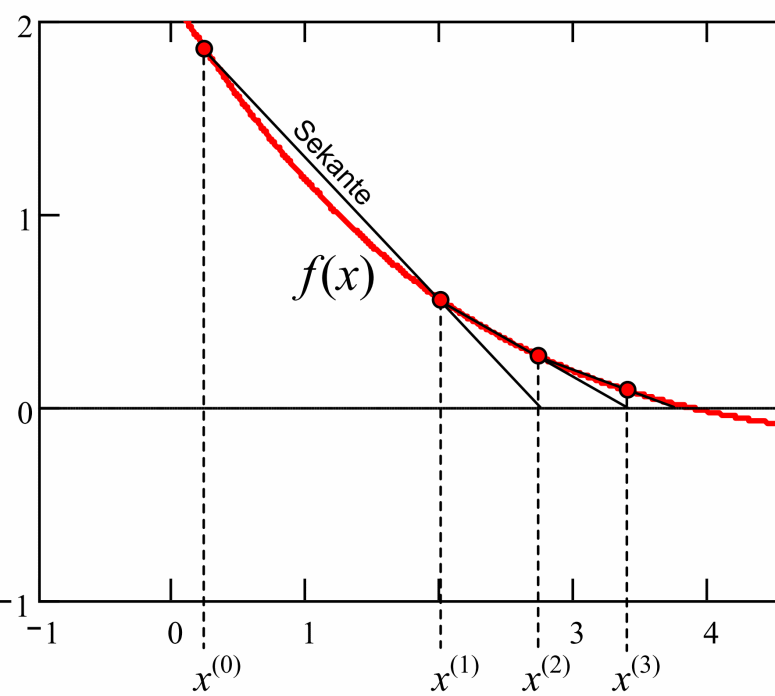
\includegraphics[width=6cm]{./Content/NonLinearOptimization/QuasiNewton1D.png}
   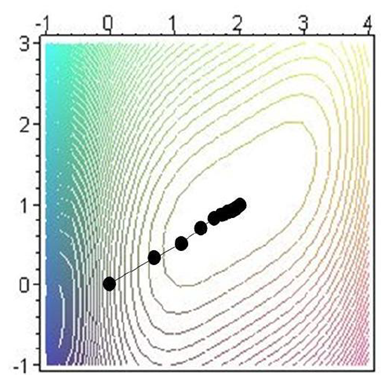
\includegraphics[width=6cm]{./Content/NonLinearOptimization/newton.png}
\end{minipage}


  Um die Berechnung der Ableitungen zu umgehen, werden diese durch finite Differenzen approximiert. 
  $$\frac{\partial^2 f}{\partial x_i^2} = \frac{1}{\epsilon^2} 
  \left( f(x_1, x_2, \ldots, x_i+\epsilon, \ldots, x_n) - 2 f(x_1, x_2, \ldots, x_i, \ldots, x_n) + f(x_1, x_2, \ldots, x_i-\epsilon, \ldots, x_n) \right)$$
  $$\frac{\partial^2 f}{\partial x_i \partial x_j} = \frac{1}{4 \epsilon^2} \begin{pmatrix}
    f(x_1, x_2, \ldots, x_i+\epsilon, \ldots, x_k+\epsilon, \ldots, x_n) - f(x_1, x_2, \ldots, x_i-\epsilon, \ldots, x_k+\epsilon, \ldots, x_n)\\
    -f(x_1, x_2, \ldots, x_i+\epsilon, , \ldots x_k-\epsilon, \ldots, x_n) + f(x_1, x_2, \ldots, x_i-\epsilon, \ldots, x_k-\epsilon, \ldots, x_n)
  \end{pmatrix}$$
 
 \subsection{Konvergenzbeschleunigung\skript{17}}
 \textbf{Idee:} Mit der sogenannten Aitken'sche   $\nabla^2$–Methode wird aus der Folge $\{x_i\}$ die die schneller konvergierende Folge $\{\hat{x}_i\}$ berechnet.\\
 
 Aitken $\nabla^2$-Methode:\quad $\boxed{\hat{x}=x_i-\frac{(x_{i+1}-x_i)^2}{x_{i+2}-2x_{i+1}+x_{i}}}$\qquad $i\geq 0$ \qquad (Formel dimensionsweise anwenden, für $x_1$, $x_2$, $\ldots$)
 
 
 

  

\section{Graphen und Netzwerke}
\begin{tabularx}{\textwidth}{p{4cm} X}
  Exakter Algorithmus
    & Findet optimale Lösung\\
  Heuristik
    & Findet gute, aber normalerweise nicht optimale Lösung\\
  Greedy Algorithmus
    & Trifft zu jedem Zeitpunkt aktuell beste Wahl, d.h. lokales Optimum; müssen nicht zu globalen Optimum führen \\
  Ungerichteter Graph
    & Graph mit endlicher Menge Ecken $V$ und Kanten $v,w \in E$\\
  Einfacher Graph
    & Keine Schlingen, keine parallelen Kanten \\
  Schlinge
    & Kante, wo Anfang- gleich Endecke ist ($vv$)\\
  Pfad 
    & Folge von Ecken $v_0, v_1, ... v_k$\\
  Kreis 
    & Pfad, wo die Anfangsecke gleich der Endecke: $v_0 = v_k$\\
  Azyklischer Graph, Wald
    & Graph, der keinen Kreis enthält\\
  Baum
    & Azyklischer, zusammenhängender Graph\\
  Bipartiter Graph
    & Die Ecken können in zwei Teilmengen aufgeteilt werden, so dass jede Kante je eine Ecke in beiden Teilmengen hat \skript{10}\\
  Eulerkreis
    & Kreis, der jede Kante des Graphen genau ein Mal enthält\\
  Hamiltonkreis
    & Kreis, der alle Ecken genau ein Mal besucht und zudem in der Startecke startet und endet\\
  Euler-/Hamiltongraph
    & Wenn Graph einen Euler- oder Hamiltonkreis enthält\\
\end{tabularx}


\subsection{Repräsentation von Graphen \skript{3}}
  
\begin{center}
	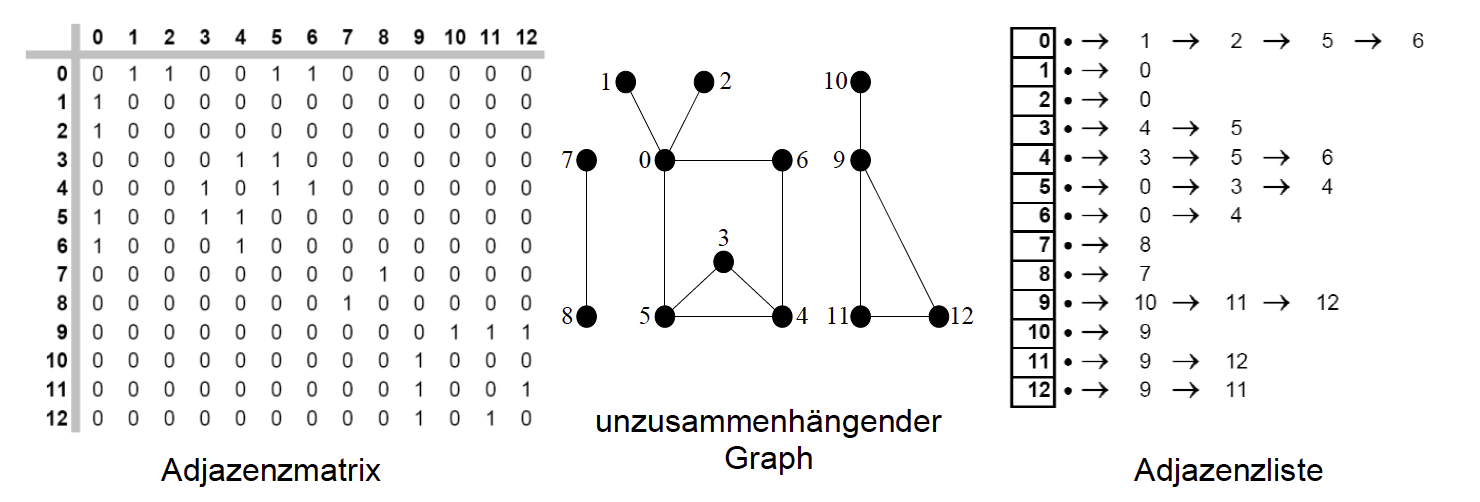
\includegraphics[width=0.8\textwidth]{Content/Graphen/AdjListMatrix.png}
	  
	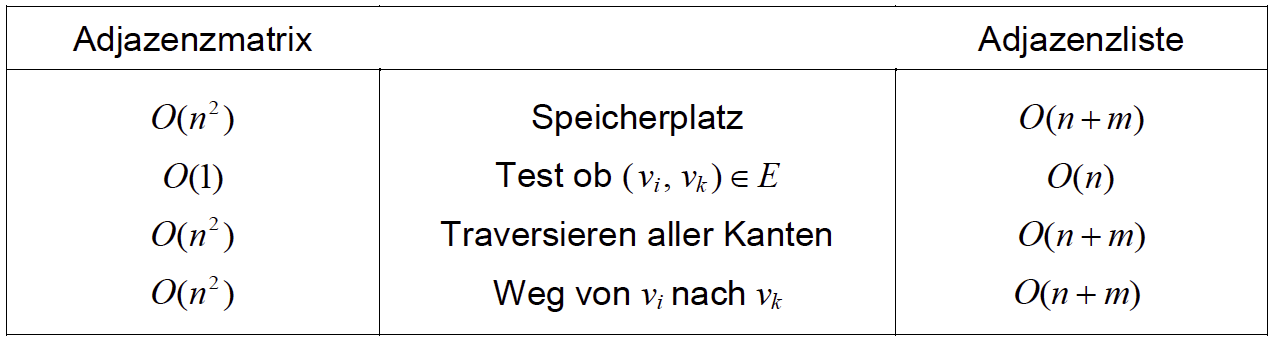
\includegraphics[width=0.5\textwidth]{Content/Graphen/KomplAdj.png}
\end{center}


\subsection{Entscheidungsbaum-Verfahren \skript{4}}
	Das Travelling-Salesman-Problem (\skript{31}), wo jede Stadt genau ein Mal besucht werden darf, ist lösbar mit dem Branch-And-Bound Verfahren.


\subsection{Traversieren von Graphen \skript{9}}

\begin{minipage}{0.5\textwidth}
	\subsubsection{Tiefensuche (Depth-First Search, DFS)}
		Ausgehend von einer Ecke, wird immer weiter zur nächsten Ecke durch den Baum "traversiert", bis das Ende erreicht ist. Dann wird von der nächsten unbesuchten Ecke weitertraversiert, bis alle Ecken besucht sind. Dies ist eine Last-In-First-Out (LIFO) Strategie.
		
		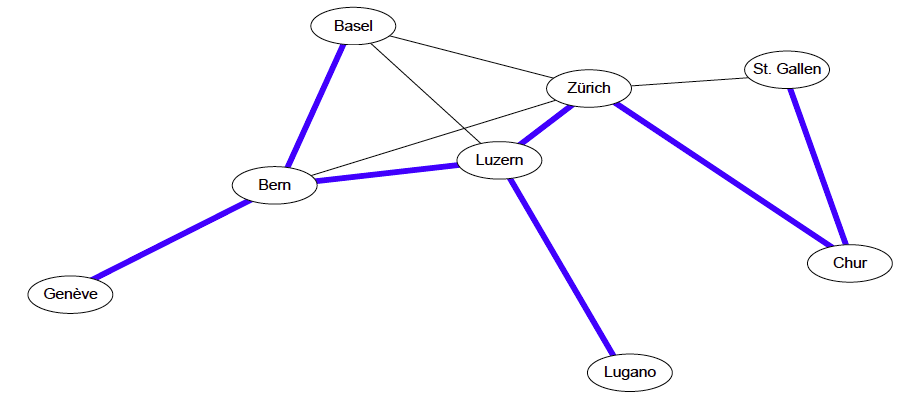
\includegraphics[width=\textwidth]{Content/Graphen/DFS.png}
		\begin{center}
		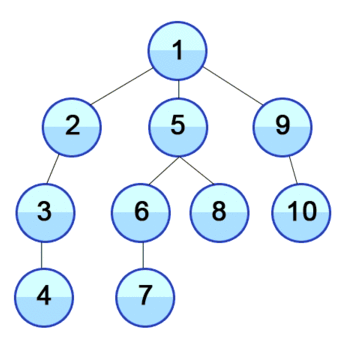
\includegraphics[width=0.3\textwidth]{Content/Graphen/tiefensuche.png}\\
		Output: 4,3,2,7,6,8,5,10,9,1\end{center}
\end{minipage}
\begin{minipage}{0.5\textwidth}
	\subsubsection{Breitensuche (Breadth-First Search, BFS)}
	  	Von einer Ecke werden alle benachbarten Ecken aufgesucht und im nächsten Schritt einer dieser benachbarten Ecken besucht. Dies ist eine First-In-First-Out (FIFO) Strategie.
	  	
	  	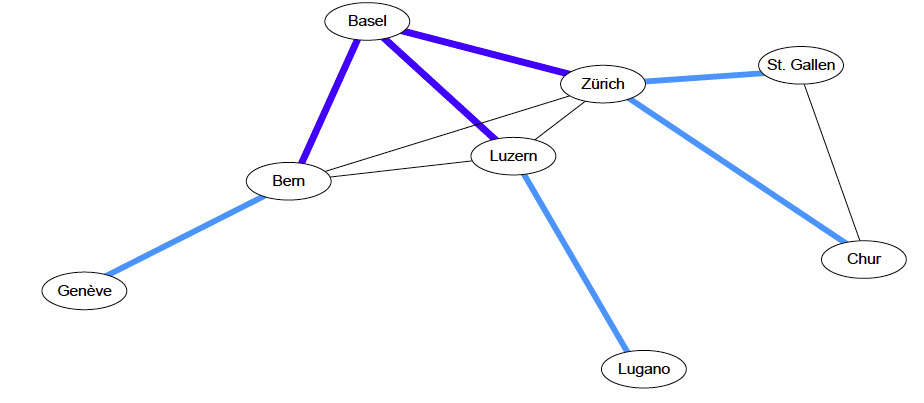
\includegraphics[width=\textwidth]{Content/Graphen/BFS.png}  
	  	\begin{center}
	  	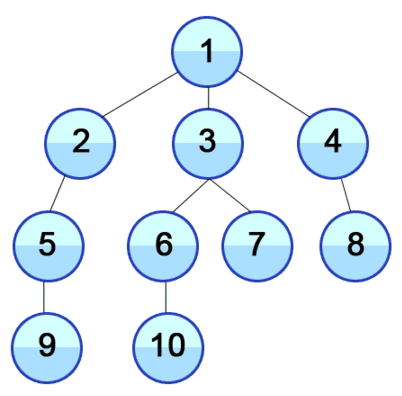
\includegraphics[width=0.3\textwidth]{Content/Graphen/breitensuche.png}\\
	  	Output: 1,2,3,4,5,6,7,8,9,10
	  	\end{center}
\end{minipage}

	
% MSTs
\subsection{Minimum Spanning Tree (MST)}

MST = Aufstellen eines Minimalen Baums: Summe aller Kantengewichte ist minimal unter allen verbundenen Knoten.
	
	\begin{tabularx}{\textwidth}{p{4cm} X p{4cm}}
	  \textbf{Prim}-Algorithmus
	    & Läuft über Ecken, ist greedy
	    & $O(n^2)$ \\
	  \textbf{Kruskal}-Algorithmus
	    & Läuft über Kanten, ist greedy
	    & $O(m \log(m))$\\
	  \textbf{MST-Heuristik} zur Lö\-sung des TSP
	    & Von bestehendem MST aus, wird in beliebige Richtung iteriert
	    & $O(n)$ ??
	\end{tabularx}


\subsubsection{Prim-Algorithmus}
Setzt Ecken ($O(n^2)$) Zwischengraph ist immer zusammenhängend.
\begin{enumerate}
	\item Beliebige Startecke $v_0$ für den MST wählen
	\item Ecke $v_i$ mit kleinstem Abstand zu einer Ecke im MST hinzufügen
	\item Punkt 2 wiederholen bis alle Ecken im MST
\end{enumerate}


\subsubsection{Kruskal-Algorithmus}
Setzt Kanten ($O(m \log(m))$) Zwischengraph ist allenfalls unzusammenhängend.
\begin{enumerate}
	\item Kante mit kleinstem Gewicht in den MST aufnehmen
	\item Kante $e_i$ mit kleinstem Gewicht, die zwei Ecken verbindet die noch nicht durch den MST verbunden sind, im MST aufnehmen
	\item zu 2 bis alle Ecken verbunden sind
\end{enumerate}


\subsubsection{MST-Heuristik zur Lösung des TSP}
Generiert Hamiltonkreis (Lösung des TSP) aus MST (Lösung muss nicht optimal sein!, Lösung ist abhängig vom Startpunkt)

\begin{enumerate}
	\item Jede Kante im MST verdoppeln (Eulergraphen)
	\item Eulerkreis auswählen (durchläuft alle Kanten)
	\item Eulerkreis durchlaufen und dabei alle bereits besuchten Knoten überspringen (Hamiltonkreis)
\end{enumerate}


% Minimaler Weg
\subsection{Minimaler Weg}

\subsubsection{Probleme}
    \begin{tabular}{ll}
      Source-sink shortest path
        & Kürzesten Weg zwischen einer Ecke (Quelle/source) und einer andern Ecke (Senke/sink) \\
      Single source shortest paths
        & Kürzeste Wege von einer Ecke (Quelle/source) zu allen anderen Ecken \\
      All pairs shortest paths
        & Kürzeste Wege zwischen allen Eckenpaaren\\
    \end{tabular}
  \subsubsection{Algorithmen}
    \begin{tabularx}{\textwidth}{p{3cm} p{4cm} X r}
      \textbf{Algorithmus} & \textbf{Löst} & \textbf{Bemerkungen} & \textbf{Compl.} \\
      \hline
      \textbf{Dijkstra} \skript{14} 
        & Source-sink shortest path, single source shortest path
        & Kantengewichte $\omega(v_i v_j) \geq 0$; Greedy; Loop über alle bereits besuchten Ecken: Suche minimale Distanz zu nächster Ecke. Der Weg, der am Schnellsten am Ziel ist, gewinnt.
        & $O(n^2)$\\
      \hline
      \textbf{Bellman-Ford}
        & Source-sink shortest path, single source shortest path
        & Auch negative Kantengewichte möglich; n~Knoten, m~Kanten
        & $O(n\cdot m)$\\
      \hline
      \textbf{A*} 
        & Single source shortest path
        & Heuristische Methode des Dijkstra, beschleunigte Laufzeit, findet optimale Lösung, benötigt viel(!) Speicher
        & ?\\
      \hline
      \textbf{Floyd-Warshall} \skript{16}
        & All pairs shortest paths 
        & Gerichtete Kreise möglich, Kantengewichte $\omega(v_i v_j) \geq 0$
        & $O(n^3)$\\
      \hline
    \end{tabularx}
    
    
\subsubsection{Dijkstra}
Sucht die kürzeste Verbindung zwischen Knoten $v_0$ und $v_n$ Kantengewicht müssen positiv sein! (sonst kann es zu nicht-optimalen Lösungen führen, da ein nicht beachteter Umweg schlussendlich kürzer gewesen wäre)
Die Menge $V$ enthält alle Ecken die bereits erreicht wurden.
$l_i$ ist der kürzeste Weg von der Ecke $v_0$ zur Ecke $v_i$.

\begin{enumerate}
	\item Beliebige Startecke $v_0$ wählen und in die Ecken-Menge $V$ aufnehmen
	\item Aus den von $V$ direkt erreichbaren Ecken diejenige zu $V$ hinzufügen, die zu $v_0$ die kürzeste Distanz hat
	%\item Diejenige Ecke zu $V$ hinzufügen, die mit dem kleinsten Abstand $w$ (von $v_0$ aus gemessen) von einer Ecke in $V$ erreicht wird
	\item $l_j = l_i + w$ ($j$ ist die neue Ecke und $i$ die Ecke, die bereits in $V$ ist, $w$ ist die Distanz zwischen $i$ und $j$)
	\item Gehe zu 2 bis die Ecke $v_n$ zu $V$ hinzugefügt wird
\end{enumerate}

\begin{center}
	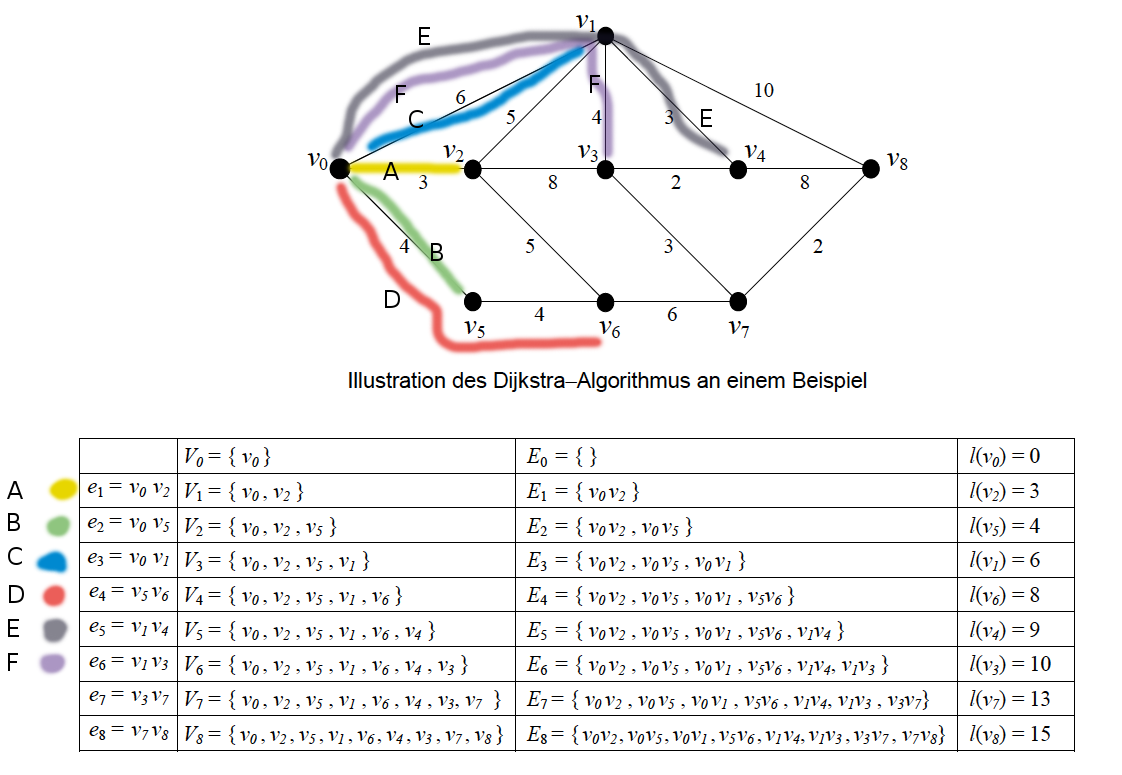
\includegraphics[width=0.8\textwidth]{Content/Graphen/Dijkstra.png}
\end{center}


\subsubsection{A*}
Der A*-Algo. untersucht immer die Koten zuerst, die wahrscheinlich schnell zum Ziel führen. Diese Wahrscheinlichkeit wird ermittelt, in dem jedem bekannten Knoten $x$ ein Wert $f(x)$ zugewiesen wird. $f(x)$ beschreibt die Distanz vom Start zum Ziel über den verwendeten Knoten ist. Der Knoten mit dem kleinsten $f(x)$ wird als nächster untersucht.
\[ f(x) = g(x) + h(x) \qquad \qquad g(x): \text{ Weg vom Startknoten bis zu }x  \qquad h(x): \text{ Weg von $x$ zum Zielknoten (Heuristik)}\]
Eine Heuristik für die Verbindung von Städten wäre z.B. die Luftlinie. Für die Durchführung des Algos wird eine \textbf{Closed-List} (untersuchte Knoten) und eine \textbf{Open-List} (gefundene, aber noch nicht untersuchte Knoten) verwendet. \textbf{Gefundene Knoten} sind, die die eine Verbindung mit einem Knoten der Closed-List haben.\\

\textbf{Bsp.:} Gesucht ist der kürzeste Weg von $Post$ nach $A$.
Bei diesem Beispiel wird für die Distanzheuristik $h(x)$ zwischen den Knoten $v_i$ und $v_j$ der Betrag $h(x)=|\textcolor{red}{i}-\textcolor{red}{j}|$ verwendet ((\textcolor{red}{rot}) $A=1$, $B=2$, etc.).

\begin{minipage}{0.5\textwidth}
	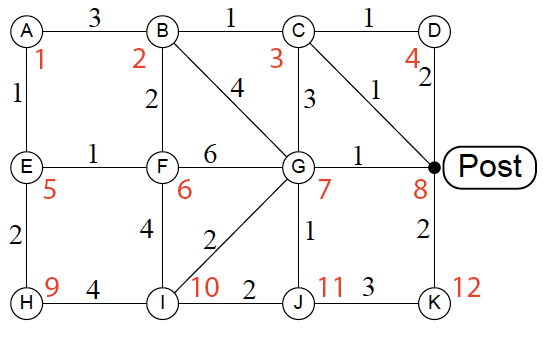
\includegraphics[width=\textwidth]{Content/Graphen/PostAStar.png}
\end{minipage}
\hfill
\begin{minipage}{0.5\textwidth}
	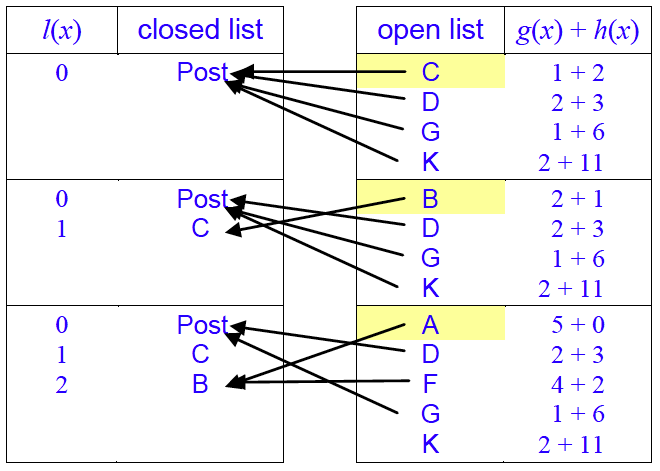
\includegraphics[width=\textwidth]{Content/Graphen/AStar.png}
\end{minipage}

Der Minimale Weg von der Post zum Knoten A beträgt 5 und kann rückwärts rekonstruiert werden:\\ $A\rightarrow B\rightarrow C \rightarrow Post$\\

\subsubsection{Floyd-Warshall}
Alle Kreise müssen ein nicht negatives Gewicht haben! Der Algorithmus ist konzipiert für gerichtete Graphen, funktioniert auch für ungerichtete (beide Richtungen gleiches Gewicht).

$shortestPath(i,j,k)$ gibt den kürzesten weg vom Knoten $v_i$ nach $v_j$, wobei der Weg über die ersten $k$ Knoten führen kann ($v_0,...,v_{k-1}$).

Die Funktion kann rekursiv implementiert werden:
\[ shortestPath(i,j,k+1) = \min \begin{cases} shortestPath(i,j,k) \qquad \qquad \qquad \qquad \qquad \text{Weg bereits bekannt (führt über $v_0, \ldots, v_{k-1}$)}\\ shortestPath(i,k,k)+shortestPath(k,j,k) \qquad  \text{Weg führt über $k$ und von dort nach $j$} \end{cases} \]

Hat ein Graph keine Kante von $v_i$ nach $v_j$ dann wird das Gewicht auf $\infty$ gesetzt!

Das Resultat des Algos ist eine Matrix, in der die kürzesten Distanzen zwischen allen Knoten angegeben ist.

\begin{enumerate}
	\item Init: setze $shortestPath(i,j,0)$ (Pfade von $v_i$ nach $v_j$ ohne Zwischenknoten)
	\item entwickle $shortestPath(i,j,k+1)$ für $k=0,1,...,n-1$ rekursive (überschreiben der Elemente bei kürzerem Weg)
	\item Matrix enthält alle kürzesten Wege
\end{enumerate}

\textbf{Bsp.:} (nichts eingetragen $=\infty$)

\begin{minipage}{0.5\textwidth}
	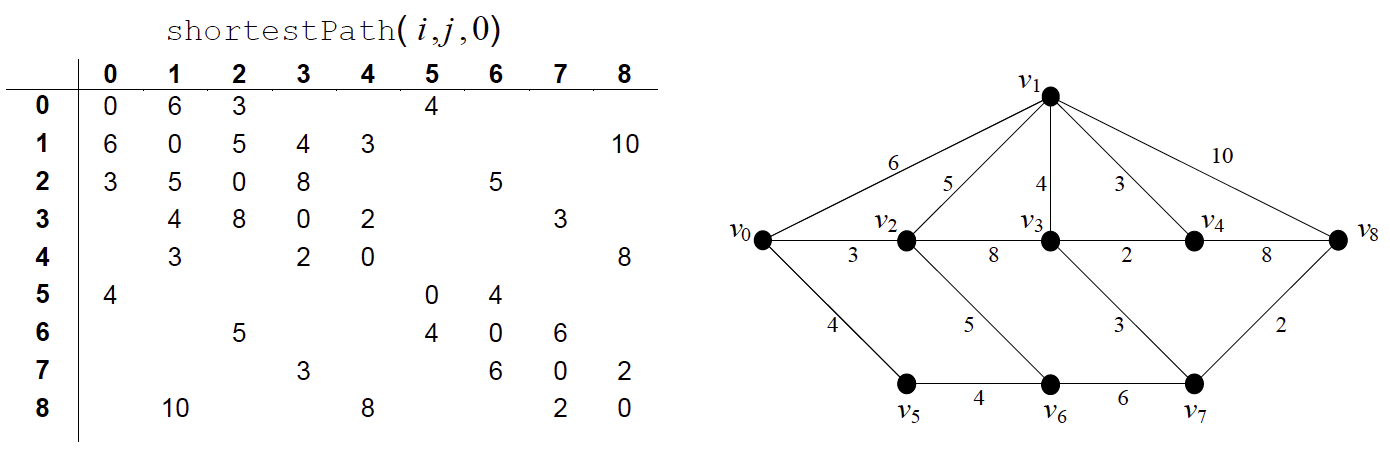
\includegraphics[width=\textwidth]{Content/Graphen/FloydWarshall1.png}
\end{minipage}
\begin{minipage}{0.5\textwidth}
	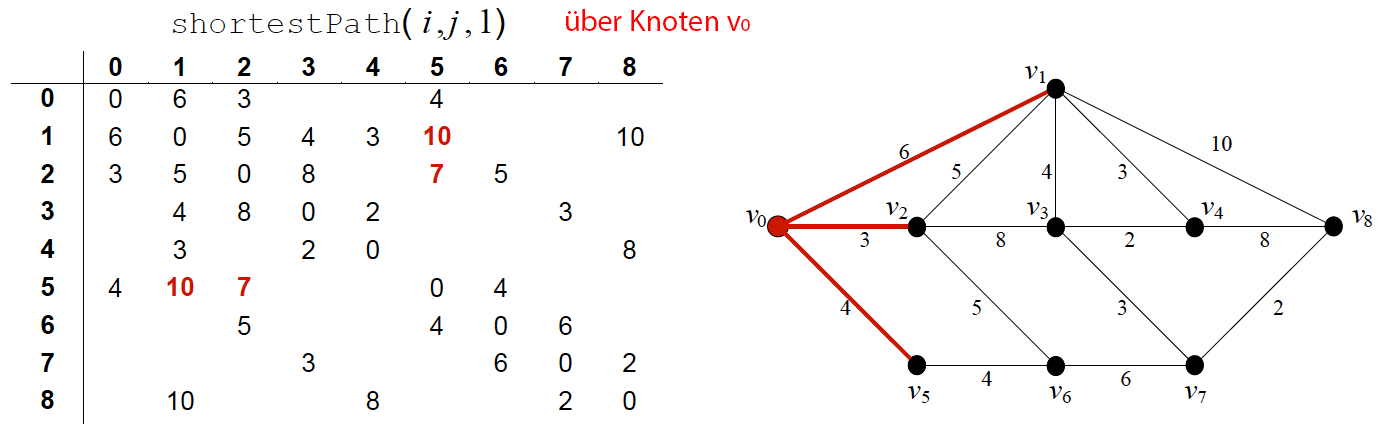
\includegraphics[width=\textwidth]{Content/Graphen/FloydWarshall2.png}
\end{minipage}
\begin{minipage}{0.5\textwidth}
	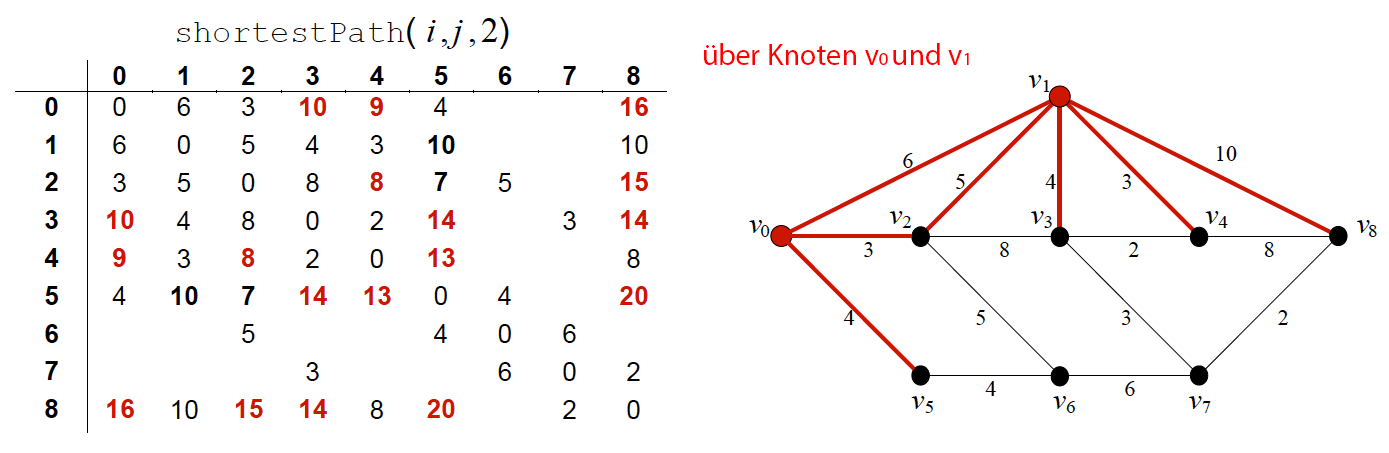
\includegraphics[width=\textwidth]{Content/Graphen/FloydWarshall3.png}
\end{minipage}
\begin{minipage}{0.5\textwidth}
	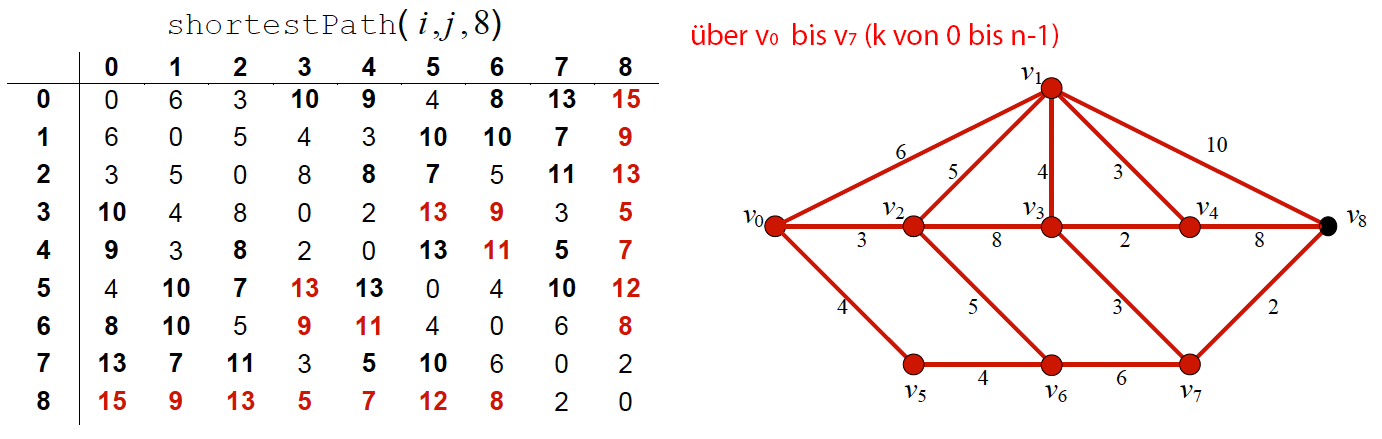
\includegraphics[width=\textwidth]{Content/Graphen/FloydWarshall4.png}
\end{minipage}

Aus der resultierenden Matrix kann nicht nur der kürzeste sondern auch der längste Pfad entnommen werden. Dieser wird auch Durchmesser des Graphen genannt.


%
% Netzwerke
%
\section{Netzwerke}
Jede Kante $vw$ hat jetzt auch eine Kapazität $c(vw)$, welche eine Obergrenze für den Fluss $f(vw)$ darstellt. Zusätzlich können den Kanten noch Kosten $k(vw)$ angefügt werden.
  
  \begin{tabularx}{\textwidth}{l X}
    Verteilungsproblem
      & Objekte von einem oder mehreren Orten (sources) an eines oder mehrere Ziele (sinks) zu verteilen\\
    Matching-Probleme
      & Zuordnung von Mengen, kann auch als bipartite Graphen interpretiert werden (bspw. Partnervermittlung) \\
    Schnitt-Probleme
      & Kanten entferne, um Netzwerk zu zerlegen (bspw. max. Anzahl Unterbrüche in Kommunikationsnetz)\\
  \end{tabularx}

% Reduktion auf Maxflow-Problem
\subsection{Reduktion auf Maxflow-Problem}

Viele bestehenden Probleme können auf Maxflow-Probleme reduziert werden.
 

\begin{minipage}{0.6\textwidth}
\textbf{Mehrere Quellen / Mehrere Senken} (Übung II.5/1):\\
	\begin{enumerate}
		\itemsep-1mm
		\item Neue Quelle $s$ einführen (Kantenkapazitäten $c_s$ entsprechen der Summe der wegführenden Kapazitäten)
		\item Neue Senke $t$ einführen (Kantenkapazitäten $c_t$ entsprechen der Summe der hinführenden Kapazitäten)
	\end{enumerate}
\end{minipage}
\begin{minipage}{0.4\textwidth}
	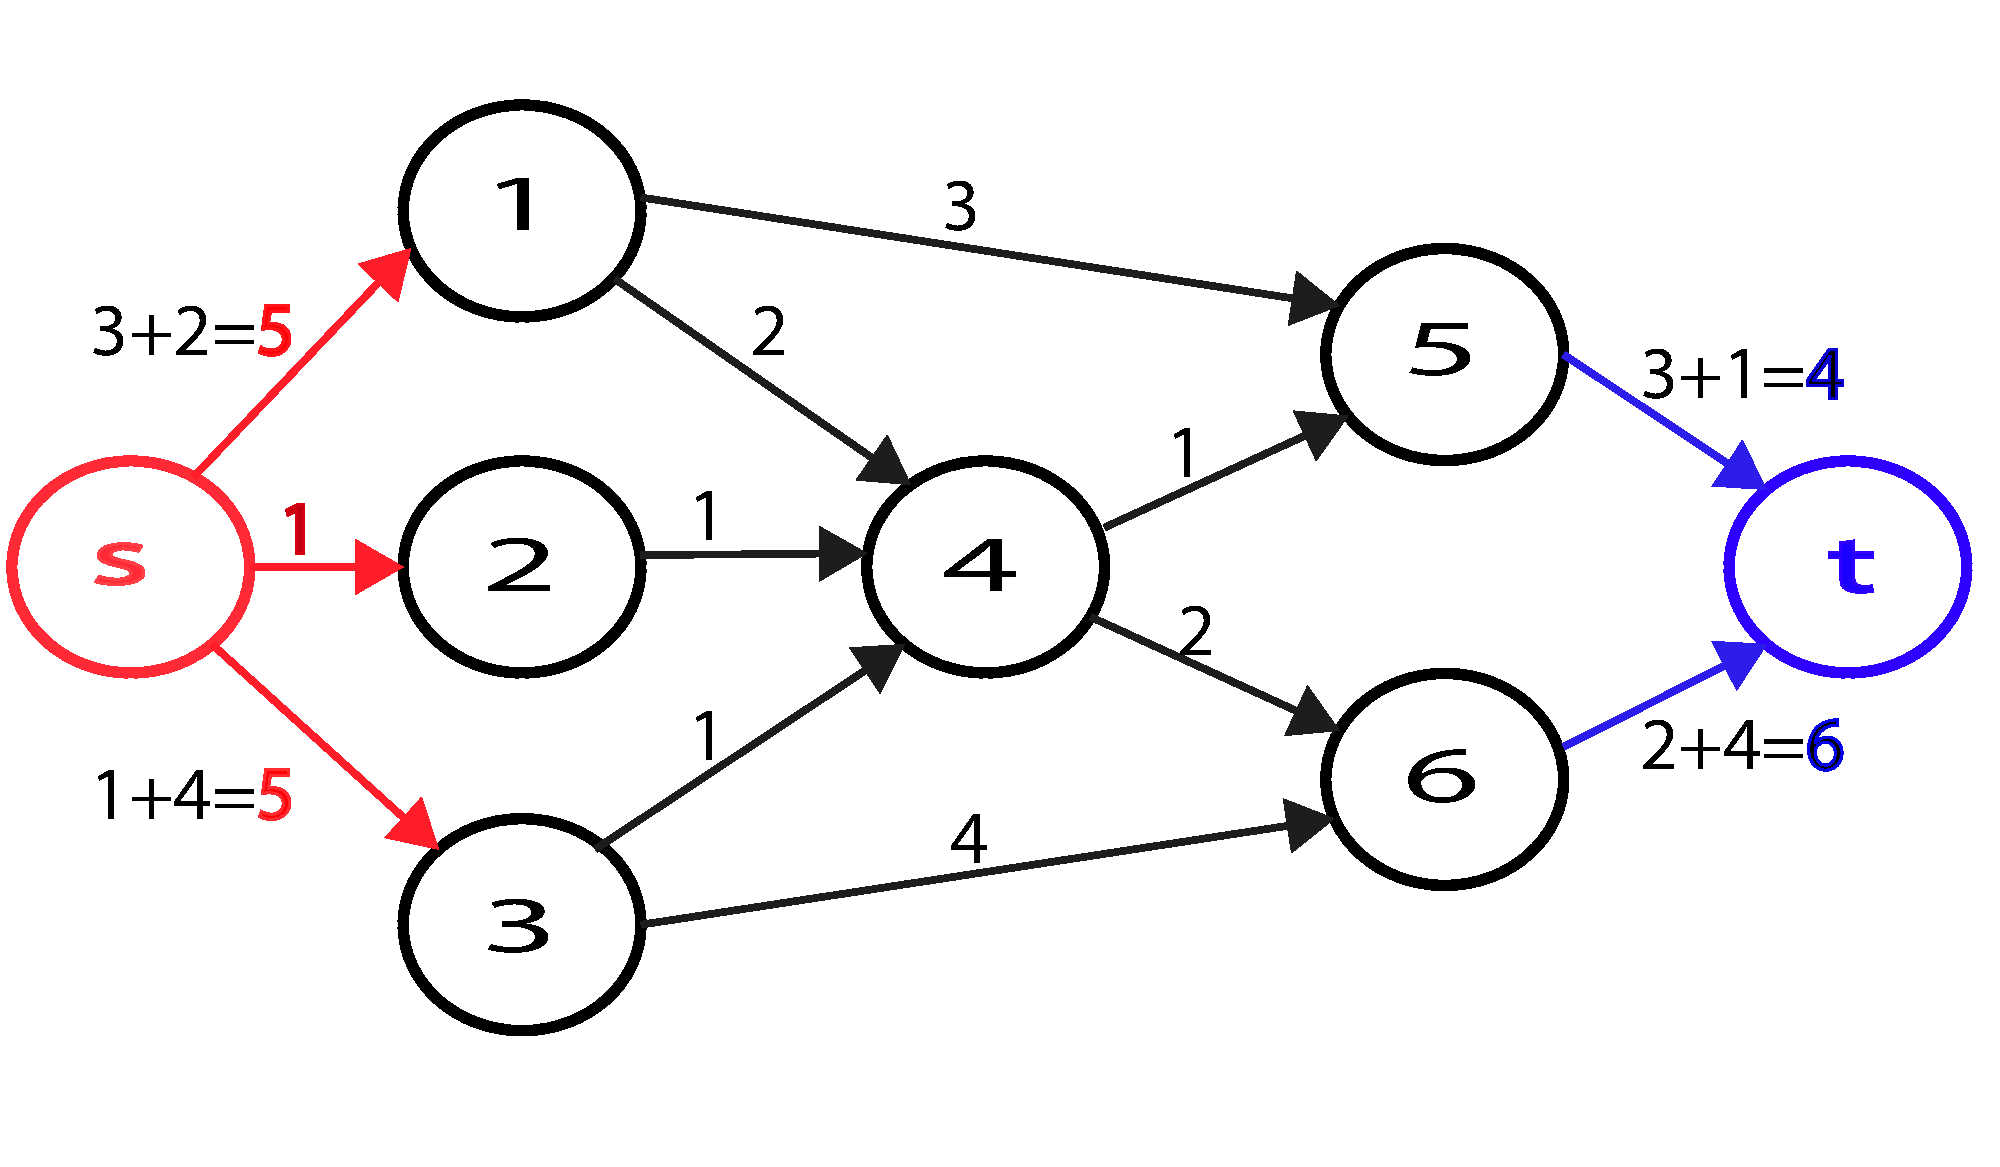
\includegraphics[width=\textwidth]{Content/Graphen/MultiSrcSink.pdf}
\end{minipage}

\textbf{Einschränkung durch Maximalkapazität:}\\
Begrenzungen durch Einführen von zusätzlichen Knoten.

\begin{minipage}{0.6\textwidth}
	\textbf{Begrenzte Output-Kapazität:}\\
	
	Neuen Knoten einführen (Kantenkapazitäten $c$ entspricht der beschränkten Output-Kapazitäten)
\end{minipage}
\begin{minipage}{0.4\textwidth}
	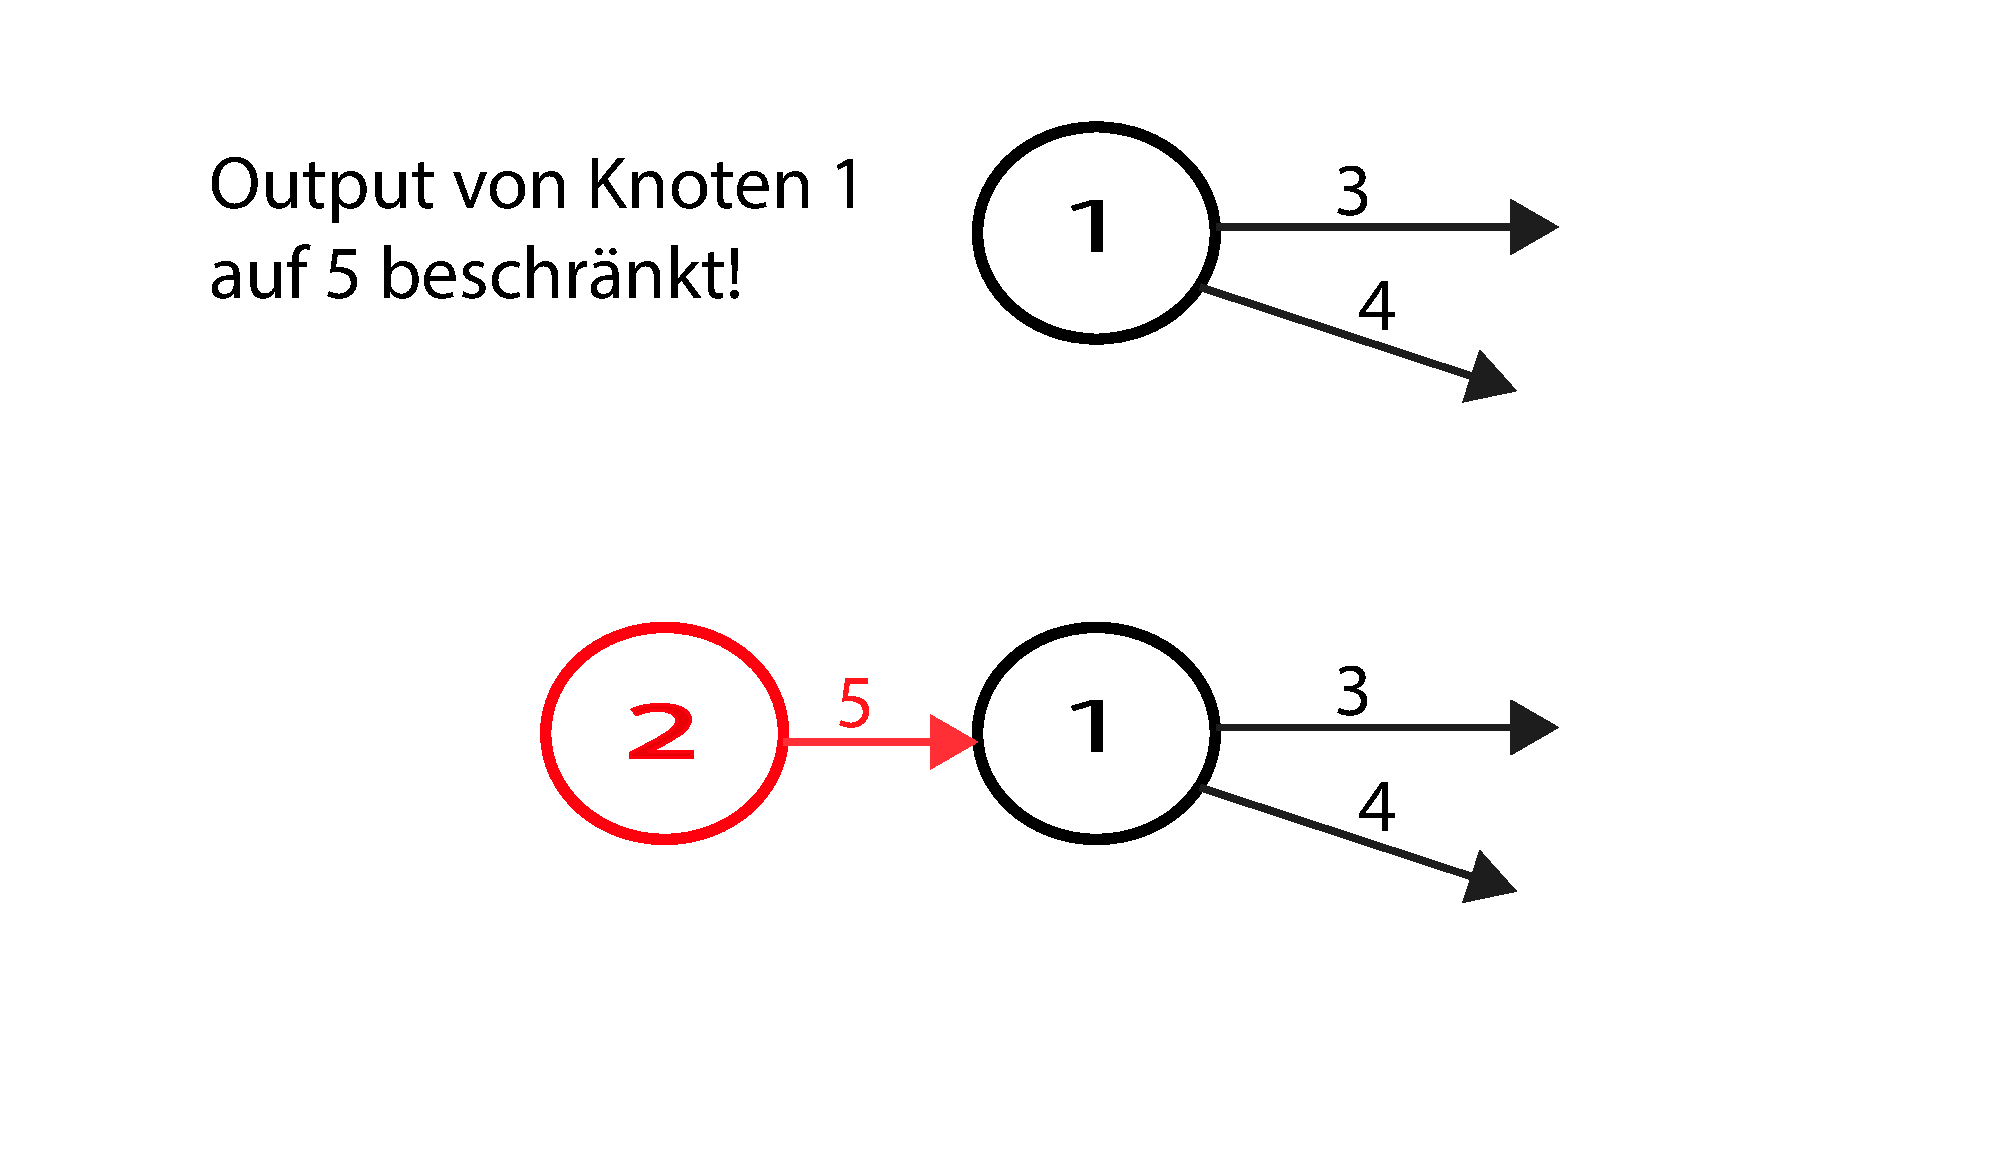
\includegraphics[width=\textwidth]{Content/Graphen/Constrain.pdf}
\end{minipage}

\begin{minipage}{0.33\textwidth}
	\textbf{Logistik-Problem} (Übung II.5/2):\\
	
	Lieferanten 0, 1, 2 haben eine Angebotskapazität\\
	Bezüger 3, 4, 5 haben eine Nachfrage\\
	neu eingefügte Quelle $s$ und Senke $t$ versorgen die Anbieter bzw. Bezüger mit den Angebot- bzw. Nachfragekapazitäten
\end{minipage}
\begin{minipage}{0.33\textwidth}
	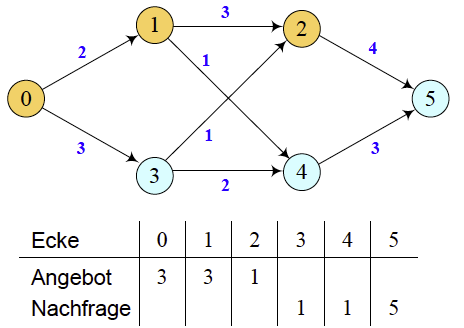
\includegraphics[width=\textwidth]{Content/Graphen/LogProb1.png}
\end{minipage}
\begin{minipage}{0.33\textwidth}	
	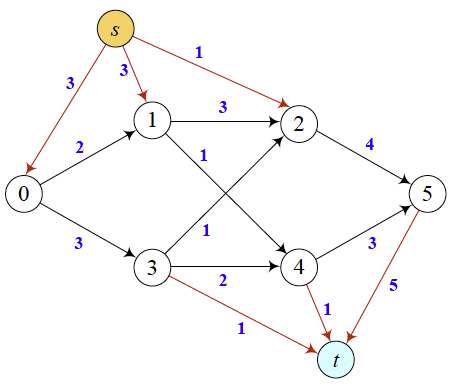
\includegraphics[width=\textwidth]{Content/Graphen/LogProb2.png}
\end{minipage}




% Maxflow Problem
\subsection{Maxflow Problem}

    Gesucht wird der maximal mögliche Fluss zwischen einer Quelle $s$ zu einer Senke $t$ ($st$-Netzwerk). Für Komplexität: $m$ = Anzahl Kanten, $f$ = maximaler Fluss von $s$ nach $t$.
    
    \begin{tabularx}{\textwidth}{p{3cm} X r}
      \textbf{Algorithmus} & \textbf{Beschreibung} & \textbf{Compl.}\\
      \hline
      \textbf{Ford-Fulkerson} \skript{22}
        & Kapazitäten müssen ganzzahlig sein! Pfade werden ausprobiert und jeweils der maximale Fluss durch diesen Pfad als (fiktiven) Rückwärtsfluss auf allen Kanten aufgetragen.
        & $O(m \cdot f)$\\
      \hline
      \textbf{Edmonds-Karp} \skript{24}
        & Gleich wie Ford-Fulkerson, aber es wird eine Breitensuche BFS angewendet.
        & $O(n\cdot m^2)$\\
      \hline
      \textbf{Max-Flow Min-Cut}
        & Der maximale Fluss in einem $st$-Netzwerk ist gleich dem minimalen Fluss über alle möglichen $st$-Schnitte.
        & -\\
      \hline
    \end{tabularx}


\subsubsection{Augmenting-Path Methode}

\begin{minipage}{0.7\textwidth}
	\begin{enumerate}
		\item Beliebigen Pfad von $s$ nach $t$ wählen
		\item Begrenzenden Teil-Pfad ermitteln; Kleinste Kapazität $f_i$ notieren
		\item Abziehen von $f_i$ von den Kapazitäten des gewählten Pfades $f_j$ ($f_j-f_i$)
		\item Wenn ein weiterer Pfad von $s$ nacht $t$ führt gehe zu  Punkt 1, andernfalls zu 5
		\item Der Gesamtfluss ist die Summe aller begrenzten Flüsse $f_{tot} = \sum_{i=1} f_i$
	\end{enumerate}
\end{minipage}
\begin{minipage}{0.3\textwidth}
	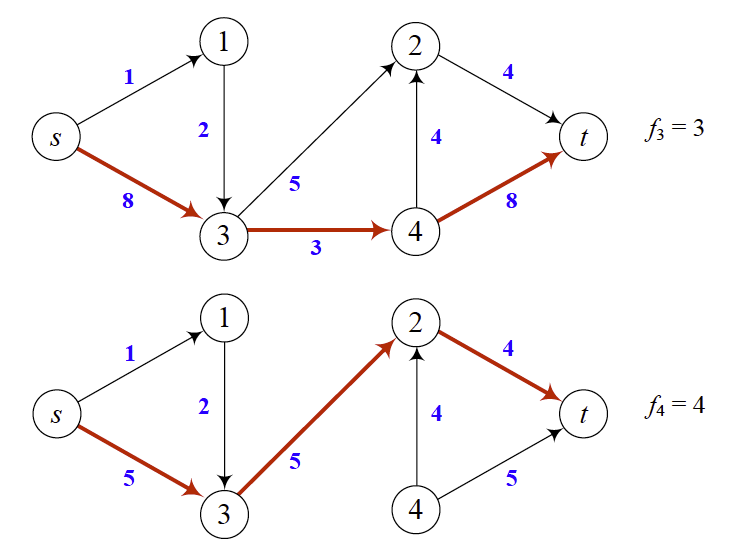
\includegraphics[width=\textwidth]{Content/Graphen/augmentingPathMethode.png}
\end{minipage}


Vorgehen ist problematisch, da es nicht möglich ist, einmal gewählte Flüsse wieder abzuwählen. (Greedy Verhalten)


\subsubsection{Ford-Fulkerson}
\begin{minipage}{0.7\textwidth}
Vorwärtspfad: Gibt an, um wieviel der Durchfluss erhöht werden kann.\\
Rückwärtspfad: Gibt an, um wieviel der Durchfluss verringert werden kann.
	\begin{enumerate}
		\item Beliebigen Pfad von $s$ nach $t$ wählen
		\item Begrenzenden Teil-Pfad ermitteln; Kleinste Kapazität $f_i$ notieren
		\item Abziehen von $f_i$ von den Vorwärtskanten $f_j$ und hinzufügen bei den Rückwärtskanten $r_j$ des gewählten Pfades $f_j$, Existiert keine Rückwärtskante muss diese eingefügt werden\\ ($f_j-f_i$ und $r_j + f_i$)
		\item Wenn ein weiterer Pfad von $s$ nach $t$ führt gehe zu  Punkt 1, andernfalls zu 5
		\item Der Gesamtfluss ist die Summe aller begrenzenden Flüsse $f_{tot} = \sum_{i=1} f_i$
	\end{enumerate}
\end{minipage}
\begin{minipage}{0.3\textwidth}
	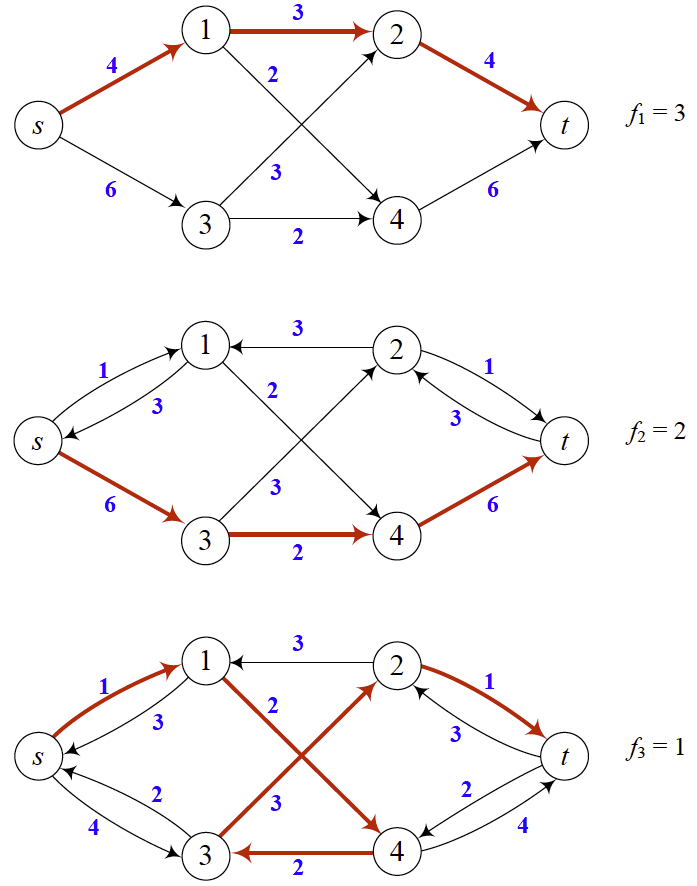
\includegraphics[width=\textwidth]{Content/Graphen/FordFulkerson.png}
\end{minipage}



\subsubsection{Max-Flow Min-Cut}
\textbf{Theorem:} \boxed{\text{Max-Flow ist gleich dem minimalen Fluss über alle möglichen ST-Cuts!}}

\begin{minipage}{0.6\textwidth}
	\textbf{Source Sink Cuts (ST-Cuts):}\\
	
	ST-Cut: Aufteilen der Ecken in eine Menge S (enthält Quelle s) und eine Menge T (enthält Senke t); $2^{|E|}$ Möglichkeiten\\
	
	Flow über ST-Cut: Summer aller Kapazitäten der Kanten, welche in S beginnen und in T enden!\\
	
	Max-Flow Min-Cut: im Bsp. ist der minimale Fluss über alle Cuts (Cut 5) gleich 7, was dem Maximalen Fluss des ST-Netzwerks entspricht.\\
	
\end{minipage}
\begin{minipage}{0.4\textwidth}
	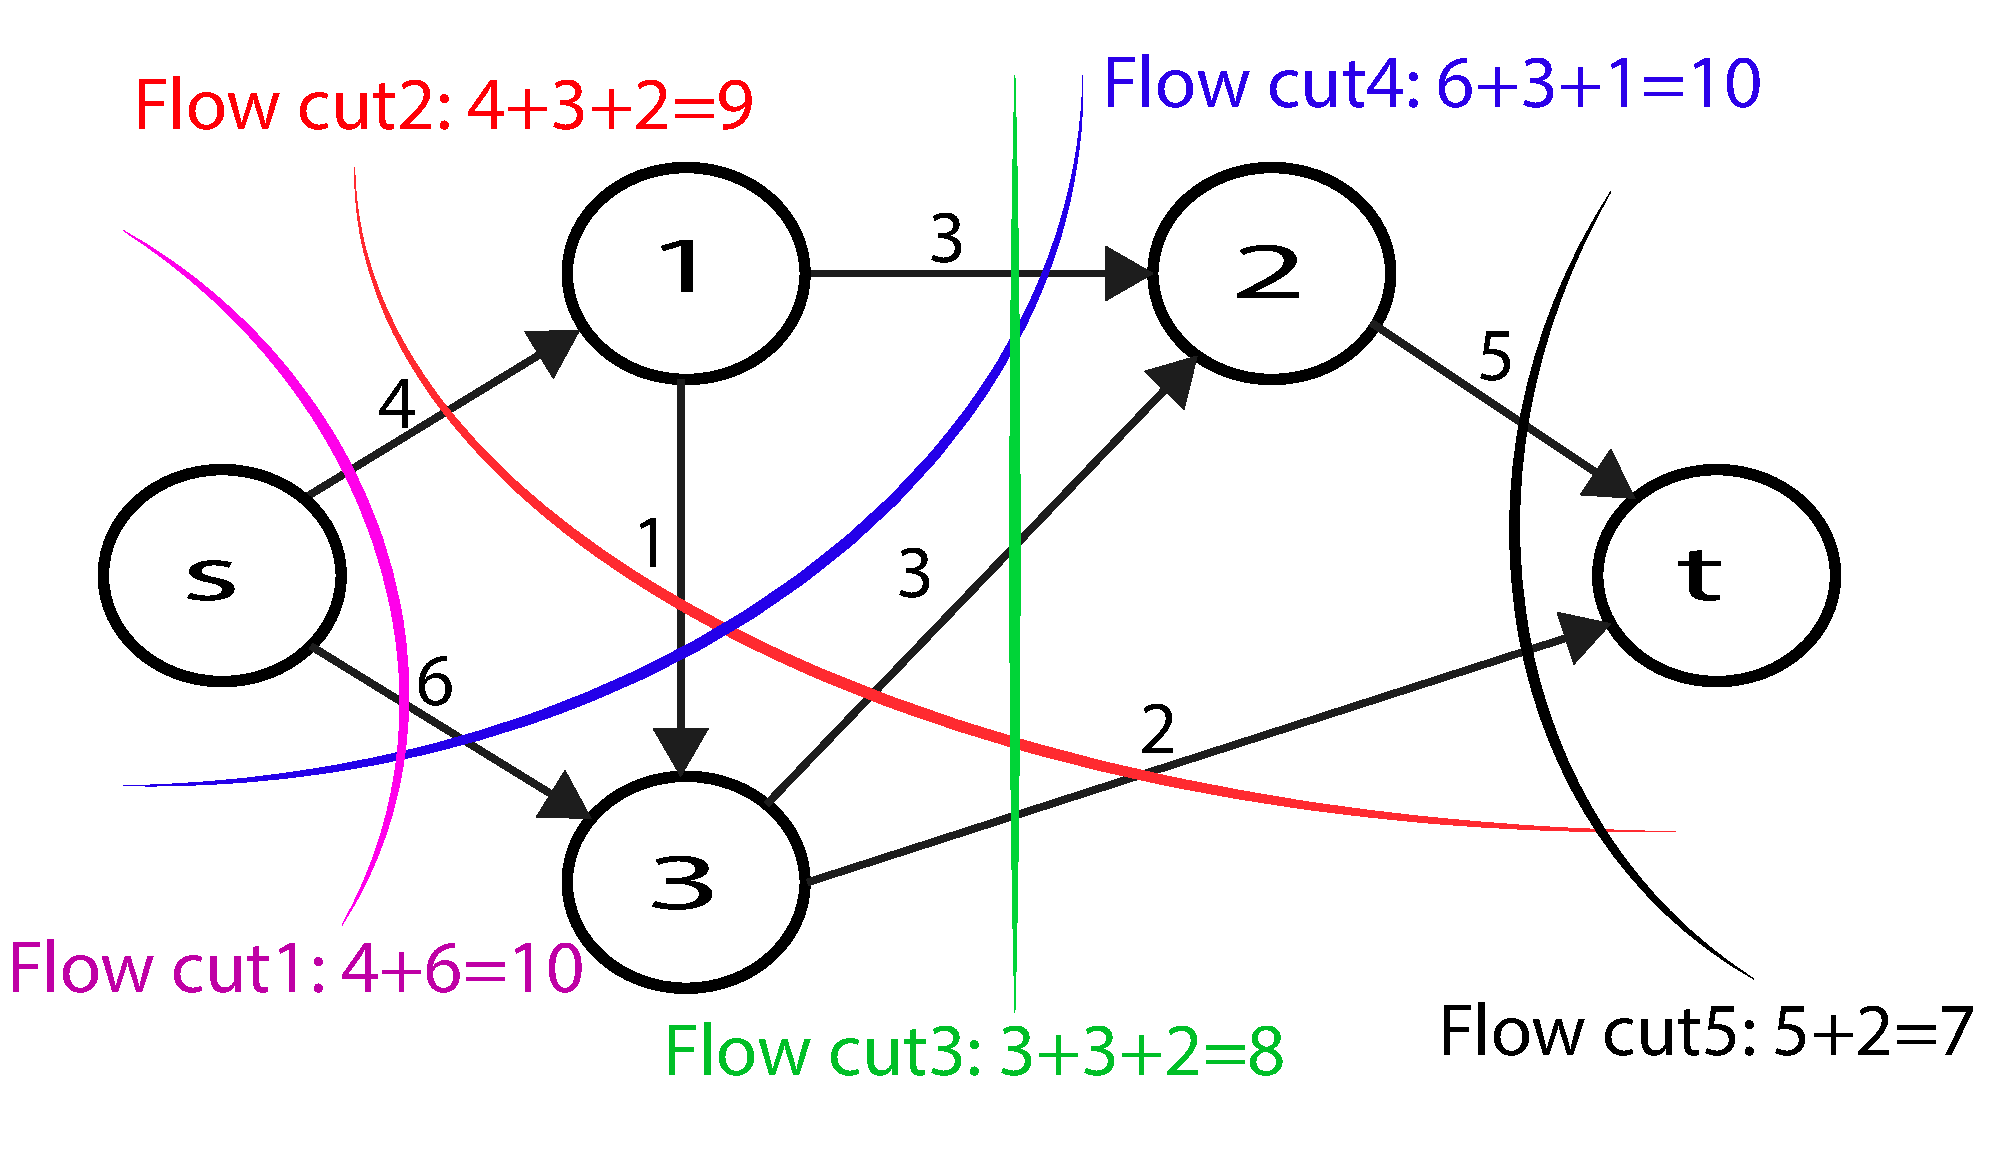
\includegraphics[width=\textwidth]{Content/Graphen/StCuts.pdf}
\end{minipage}
Min-Cut entspricht dem Nadelöhr, Max-Flow kann nur so viel sein, wie durchs Nadelöhr passt. 

% Maxflow Mincost
\subsection{Maxflow Mincost \skript{28}}
Die Lösung des Max Flow Problems ist nicht eindeutig, darum können weitere Kriterien hinzugefügt werden.\\

\textbf{Tipps:}
\begin{itemize}
\item Grosse Kreise zeichnen, damit Pfeilrichtungen eindeutig erkennbar.
\item Zweige mit geringen Transportkosten zuerst invertieren, um mit grosser Wahrscheinlichkeit negative Kreise zu unterbinden.
\end{itemize} 

\textbf{Vorgehen:}
\begin{enumerate}
	\item Ford-Fulkerson anwenden ($f_{tot}$ bleibt konstant!)
	\item Restnetzwerk durch Kantenkosten $k$ erweitern (Vorwärtskante: $+k$, Rückwärtskante: $-k$)
	\item Wenn Kreis mit negativen Kosten vorhanden gehe zu 4, andernfalls zu 5
	\item Fluss des neg. Kreises um die min. Kantenkapazität $c_{min}$ erhöhen (in Gegenrichtung!), gehe zu 3
	\item Gesamtfluss (max): $f_{tot}$ aus Ford-Fulkerson
	\item Gesamtkosten (min): Summe aller Rückwärtskantenkosten (RK) multipliziert mit der entsprechenden Kantenkapazität:\\  
	$k_{tot} = \sum\limits_{ i \in \text{alle RK}} c_i \cdot |k_i| $
\end{enumerate}

\textbf{Bsp.:}

\begin{minipage}{0.33\textwidth}
	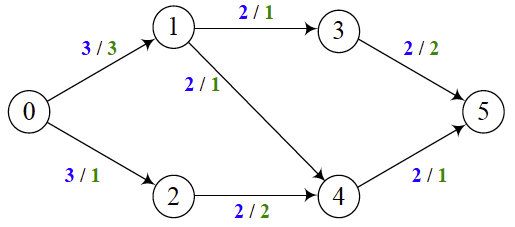
\includegraphics[width=\textwidth]{Content/Graphen/MaxFlowMinCost1.png}
	
	Ausgangsnetzwerk mit Kapazitäten\\ und Kosten
\end{minipage}
\begin{minipage}{0.33\textwidth}
	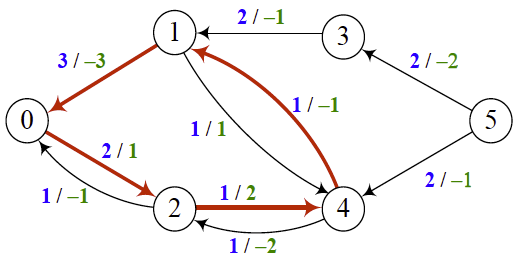
\includegraphics[width=\textwidth]{Content/Graphen/MaxFlowMinCost2.png}
	
	Restnetzwerk mit $f_{tot}=4$, $k_{tot}=21$,\\ Kreis mit neg. Kosten (rot,\\ $1+2-1-3 = -1$) mit min. Kantenkapazität $c_{min} = 1$
\end{minipage}
\begin{minipage}{0.33\textwidth}
	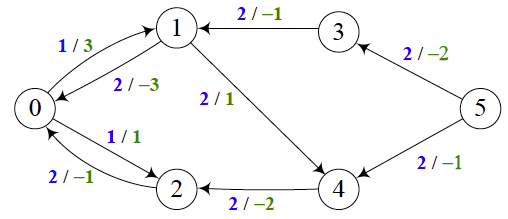
\includegraphics[width=\textwidth]{Content/Graphen/MaxFlowMinCost3.png}
	
	Neg.Kreis mit $c_{min}$ in Gegenrichtung erhöht\\
	$f_{tot} = 4$, 
	Gesamtkosten (RK!):\\ $k_{tot} = c_{1,s}\cdot|k_{1,s}| + c{2,1}\cdot|k_{2,1}|+... =\underbrace{2}_{c}\cdot\underbrace{(3+1+2+1+2+1)}_{\sum |k_i|}=20$
\end{minipage}


\section{Meta-Heuristiken}
\subsection{Hill-Climbing \skript{2}}
  Konvergiert meist in lokales Optimum, Konvergenz sehr langsam., Wahl eines Zufallsschritts ist schwierig. Zielfunktion muss oft berechnet werden.
  
  Algorithmus, um Zielfunktion $f(\vec{x})$zu maximieren:
  \begin{enumerate}
    \item Start: Wahl von $\vec{x}^{alt}$
    \item Neue Wahl $\vec{x}^{neu}$ "`in der Nähe"' von $\vec{x}^{alt}$ (zuällig)%{\tiny (Das war die komische Bitschieberei in der Vorlesung)}
    \item Wenn $f(\vec{x}^{neu}) \geq f(\vec{x}^{alt})$, setze $\vec{x}^{alt} = \vec{x}^{neu}$ und gehe zu Schritt 2
  \end{enumerate}
  
 

\subsection{Tabu-Search \skript{3}}
  Grundidee: Keine / möglichst wenige Schritte, welche die Wirkung früherer Schritte rückgängig machen.
  
  Etwas schnellere Konvergenz ggn. Hill-Climbing, allerdings aufwendiges Mitführen und Aktualisieren der Tabu-Liste sowie Schwierigkeit, um Länge der Tabu-Liste zu finden. Zielfunktion muss oft berechnet werden.
  
  Algorithmus, um Zielfunktion $f(\vec{x})$zu maximieren:
  \begin{enumerate}
    \item Start: Wahl von $\vec{x}^{alt}$
    \item Neue Wahl $\vec{x}^{neu}$ "`in der Nähe"' von $\vec{x}^{alt}$, welche mit einem erlaubten Schritt $m_i \notin T$ eine möglichst gute Verbesserung (oder geringste Verschlechterung bringt).
    \item Einfügen des komplementären Schritts $\bar{m}_i$ in Tabu-Liste $T$.
    \item Schritte 2 und 3 wiederholen, bis vorgegebenes Abbruchkriterium erreicht ist.
  \end{enumerate}

\subsection{Simulated Annealing \skript{5}}
  Grundidee: Gegenüber dem Tabu-Search wird eine Verschlechterung der Lösung mit einer gewissen Wahrscheinlichkeit akzeptiert. So kann ein lokales Optimum wieder verlassen werden.
  
  \begin{enumerate}
    \item Start: Wahl von $\vec{x}^{alt}$
    \item Neue Wahl $\vec{x}^{neu}$ "`in der Nähe"' von $\vec{x}^{alt}$
    \item Wenn $f(\vec{x}^{neu}) \geq f(\vec{x}^{alt})$ oder mit einer Wahrscheinlichkeit von $p = e^{\frac{-\Delta E}{T}}$, setze $\vec{x}^{neu} = \vec{x}^{alt}$.\\
    Metropolis Regel: Zufallsvaribale $z \in [0,1]$. Wenn $z \leq p$ dann wird der schlechtere Wert genommen $\vec{x}^{neu} = \vec{x}^{alt}$
    \item Schritte 2 und 3 wiederholen, bis vorgegebenes Abbruchkriterium erreicht ist.
  \end{enumerate}
  
  Wahl der Parameter:
  \begin{itemize}
    \item $\Delta E$: Wenn Minimum: $\Delta E = f(\vec{x}^{neu}) - f(\vec{x}^{alt})$; wenn Maximum: $\Delta E = f(\vec{x}^{alt}) - f(\vec{x}^{neu})$
    \item Veränderung der Temperatur $T(i)$ (Kühlschema): Konstant, arithmetisch (bei jedem Schritt wird um gleichen Betrag verkleinert), geometrisch (bei jedem Schritt wird um gleichen Faktor verkleinert), stufenweise (diskrete Sprünge)
    \item Anfangstemperatur $T(0)$: Z.B. mittlere Änderung der Zielfunktion über einige zufällig gewählte Schritte.
  \end{itemize}
  

\subsection{Genetische Algorithmen (GA) \skript{8}}
  
    Löst alle Klassen von schwierigen Optimierungsproblemen: Parameteroptimierungen, kombinatorische Probleme (e.g. Travelling Salesman), Subset-Selektion (Stichwort Data-Mining). Nachteile sind die Erfahrung und das Geschick, das nötig ist für deren Entwicklung.
  
    Grundprinzip: Durch \em Selektion \em (Fitness/objective function), \em Rekombination \em (Kombination des genetischen Materials der Eltern) und \em Mutation \em (Veränderung der Erbinformation) können Funktionen optimiert werden. Dabei wird iterativ von einer "`alten"' Population durch verschiedene Operationen eine neue Population generiert, welche im Normalfall gleich gross sein soll.\\
    
  \begin{minipage}{12cm}  
    Beispiel eines GA-Modells:\\
    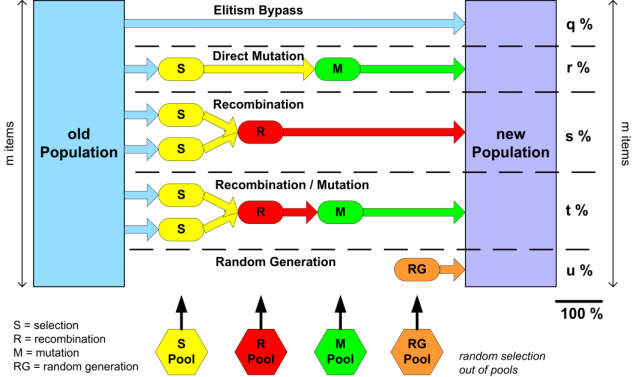
\includegraphics[width=12cm]{./Content/MetaHeuristics/GeneticAlgorithms_Model}
  \end{minipage}
  \begin{minipage}{6cm}
    \begin{flushright}
      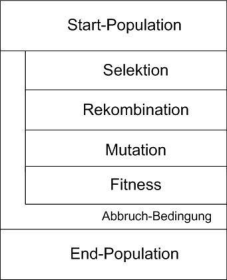
\includegraphics[width=5cm]{./Content/MetaHeuristics/GeneticAlgorithms_Principle}
    \end{flushright}
  \end{minipage}
  
  \begin{center}
    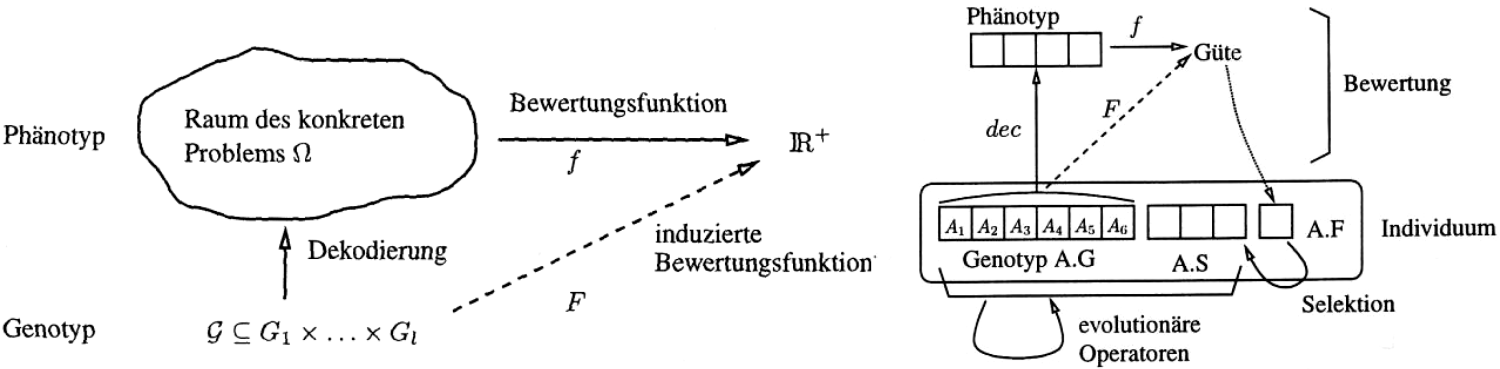
\includegraphics[width=0.7\textwidth]{./Content/MetaHeuristics/phenoGeno}
  \end{center}
  
    \subsubsection{Codierung der Parameter \skript{11}}
      Am besten werden die Parameter \em Gray\em -codiert. Damit wird erreicht, dass für jeden möglichen Parameter-Wert zwei Ein-Bit-Mutationen existieren, die den nächstgrösseren und -kleineren Parameter-Wert bilden.
      
      \begin{minipage}{0.33\textwidth}
      	\begin{center}
  	        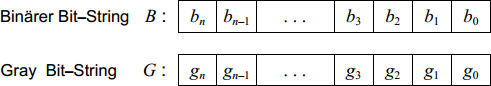
\includegraphics[width=\textwidth]{./Content/MetaHeuristics/GeneticAlgorithms_Gray}
  	      \end{center}
  	      $$g_j = \begin{cases}
  	        b_n                & j=n\\
  	        b_{j+1} \oplus b_j & j < n
  	        \end{cases} \qquad 
  	      b_j = \sum \limits_{k=n}^j \oplus g_k$$
      	\end{minipage}
      	\hfill
      	\begin{minipage}{0.3\textwidth}
            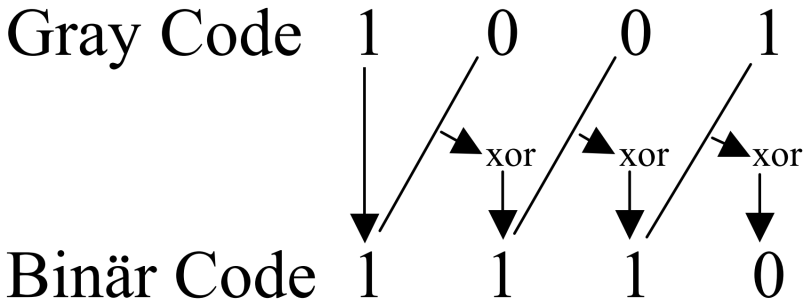
\includegraphics[width=\textwidth]{./Content/MetaHeuristics/binGray}	
    	\end{minipage}
    	\hfill
    	\begin{minipage}{0.3\textwidth}
            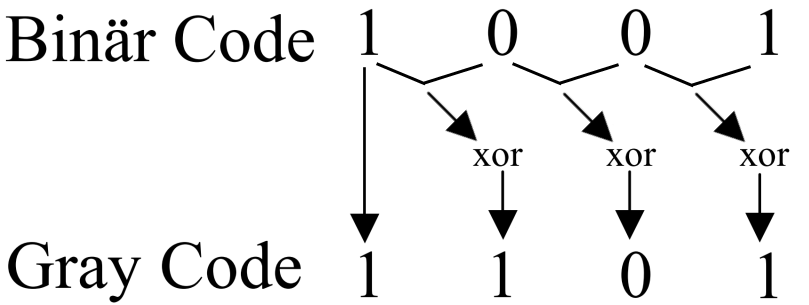
\includegraphics[width=\textwidth]{./Content/MetaHeuristics/grayBin}    	
    	\end{minipage}
  
  	Eine optimale Kodierung wurde dann vorliegen, wenn eine kleine Änderung am Genotypen eine kleine Änderung am Phänotyp bewirkt und wenn eine grosse Änderung am Genotypen auch eine grosse Änderung am Phänotyp zur Folge hat.

\subsubsection{Selektion \skript{15}}
  Probabilistische (Zufallsprinzip, z.B. \em Roulette-Wheel\em ) oder deterministische (nach Fitnesswerten, z.B. nur die besten; z.B. \em Binäre Wettkampfselektion\em ) Selektion. Problem bei beiden: Die besten Gene können verloren gehen, deshalb werden meist das beste oder die besten Individuen übernommen.
  
\subsubsection{Rekombination \skript{16}}
  \begin{tabularx}{\textwidth}{p{9cm} p{9cm}}
    \em One-Point Crossover\em : Der "`Chromosomen"'-String wird an zufälliger Stelle getrennt und neu rekombiniert: 
      & \em Two-Point Crossover\em : Der "`Chromosomen"'-String wird an zwei zufälligen Stellen getrennt und neu rekombiniert: \\
    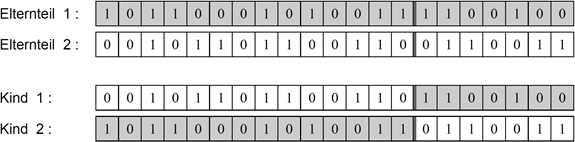
\includegraphics[width=8cm]{./Content/MetaHeuristics/GeneticAlgorithms_OnePointCrossover}
      & \includegraphics[width=8cm]{./Content/MetaHeuristics/GeneticAlgorithms_TwoPointCrossover} \\ \\
    \em $k$-Point Crossover\em : Verallgemeinerung von One-/Two-Point Crossover.
      & \em Uniform Crossover\em : $k$-Point Crossover mit Grenzwert $k \rightarrow n$, hier wird also jedes Bit zufällig kombiniert.
  \end{tabularx}
   
  
\subsubsection{Mutation \skript{18}}
  \begin{minipage}{7.75cm}
    \begin{itemize}
      \item \em Bit-Flip-Mutation\em : Zufällig ausgewählte Bits werden invertiert, wobei dies mit (kleiner) Wahrscheinlichkeit (Mutationsrate) geschieht.
      \item \em Positionsmutation\em : Bits oder ganze Bitstrings können an verschiedenen Positionen ausgetauscht werden.
      \item \em Inversion\em : Bits können auch invertiert werden (Auswahl durch Zufall).
    \end{itemize}
  \end{minipage}
  \hfill
  \begin{minipage}{10.75cm}
    \includegraphics[width=11cm]{./Content/MetaHeuristics/GeneticAlgorithms_Mutation}
  \end{minipage}
  
  \newpage
  
\subsubsection{Ersetzungsschemata \skript{19}}

  Was passiert mit der alten Population?\\
  
  
  \includegraphics[width=\linewidth]{./Content/MetaHeuristics/GeneticAlgorithms_ReplacementsCroped}
   
   
  \subsection{Ant Colony Optimization \skript{21}}
  Ameisen folgen intensiven Pheromon-Spuren, da dort die Chance auf Futter zu treffen gross ist. Diese Idee wird bei ACO aufgenommen. Mit einer Wahrscheinlichkeit $P(x_{ij})$ wird ein möglicher Pfad $ij$ in die neue Generation übernommen. Zusätzlich wird meist auch ein "`Elite-Bypass"' mit Schwellwert $Q \in [0,1]$ implementiert:
  
  $$P(x_{ij}) = \begin{cases} \dfrac{\tau_{ij}^\alpha \eta_{ij}^\beta}{\sum\limits_{j \in \mathbf{W}_i} \tau_{ij}^\alpha \eta_{ij}^\beta}  & \text{if }j \in \mathbf{W}_i\\ 0 & \text{if }j \notin \mathbf{W}_i \end{cases}
  \qquad \qquad
  P(x_{ij}) = 
  \begin{cases}
    \text{if } z < Q = 
    \begin{cases}
      1 & \text{if } j = \arg \max\limits_{k \in \mathbf{W}_i}[\tau_{ik}^\alpha \eta_{ik}^\beta] \\
      0 & \text{else}
    \end{cases} \\
    \text{if } z \geq Q
    \begin{cases}
      \dfrac{\tau_{ij^\alpha \eta_{ij}^\beta}}{\sum\limits_{j \in \mathbf{W}_i} \tau_{ij}^\alpha \eta_{ij}^\beta}  & \text{if }j \in \mathbf{W}_i\\
      0 & \text{else}
    \end{cases}
  \end{cases}$$
  
  mit $\eta_{ij}$ als heuristischer Information (z.B. Abstand $\eta_{ij} = \frac{1}{d_{ij}}$ beim TSP), $z$ ist eine gleichverteilte Zufallsvariabale im bereich $[0,1]$.
  
  Bei jedem Schritt verdunsten die Pheromone nach folgender Regel mit Verdunstungsfaktor $0 \leq \rho \leq 1$:
  $$\tau_{ij}^{neu} = \begin{cases}
    \tau_{ij}^{alt} (1-\rho) + \frac{\rho}{f(\vec{x})} & \text{if } j \in \mathbf{W}_i\\
    \tau_{ij}^{alt} (1-\rho) & \text{if } j \notin \mathbf{W}_i\\
  \end{cases}
  \qquad \qquad
  \tau_{ij}^{neu} = \varphi \cdot \tau^0 + (1-\varphi) \cdot
  \begin{cases}
      \tau_{ij}^{alt} (1-\rho) + \frac{\rho}{f(\vec{x})} & \text{if } j \in \mathbf{W}_i\\
      \tau_{ij}^{alt} (1-\rho) & \text{if } j \notin \mathbf{W}_i\\
    \end{cases}
  $$
  
  ACO kann lokalen Extremalstellen konvergieren. Die kann durch das einführnen einer Konvergenzbremse $\varphi$ abgeschwächt werden.
  
  ACO wird eingesetzt für TSP, Vehicle Routing, Graph Coloring, Routing, Scheduling, etc.
  
  ACO liefert schnell gute Resultate für kombinatorische Probleme, ist aber nicht für Parameteroptimierung geeignet.\\
  
  \lstinputlisting[language=Java]{./Content/MetaHeuristics/ACO2.java}
  
\subsection{Particle Swarm Optimization \skript{23}}
  Speziell für Parameteroptimeriung geeignet: Jedes Individuum versucht zwar, sein lokales Optimum zu finden, gleichzeitig lernt es aber von den seinen eigenen Erfahrungen und denen des Schwarms.
  
  \begin{center}
  \includegraphics[width=0.7\linewidth]{./Content/MetaHeuristics/partSwarm}
  \end{center}

\newpage
  
  \lstinputlisting[language=Java]{./Content/MetaHeuristics/PSO2.java}
  


\section{Optimization Summary}

\begin{center}
\includegraphics[width=0.7\textwidth]{./Content/OptimizationSummary/Summary}
\end{center}

\textbf{Auswahlhilfe für Algorithmen:}
  \begin{itemize}
    \item Kontinuierliche Lineare Probleme: Lineare Programmierung, Integer Programmierung
    \item Kontinuierliche nichtlineare Probleme: Gradientenverfahren (Steepest Descent, Newton) oder bei komplexeren Problemen Heuristiken (Ant Colony oder Genetische Algorithmen)
    \item Einfache/gutartige Probleme: Trajektorienbasierte Algorithmen (Hill-Climbing, Tabu Search, Simulated Annealing)
    \item Komplexe Kombinatorische Probleme: Ant Colony oder Genetische Algorithmen
    \item Komplexe Parameteroptimierungen: Particle Swarm Optimization oder Genetische Algorithmen
  \end{itemize}



\end{document}
